\documentclass[ author={Stephen Livermore-Tozer},
				supervisor={Dr. Peter Flach},
				degree={MEng},
				title={Algorithmic Co-composition Using Machine Learning},
				subtitle={},
				type={research},
				year={2016} ]{dissertation}
				
\usepackage{tikz}
\usetikzlibrary{matrix,chains,positioning,decorations.pathreplacing,arrows}
\usepackage{graphicx}
\usepackage{hyperref}
\usepackage{booktabs}
\usepackage{caption}
\usepackage{multirow}

\renewcommand{\baselinestretch}{1.15} 

\DeclareMathOperator*{\argmin}{arg\,min}
\DeclareMathOperator*{\argmax}{arg\,max}

\newcommand{\setmeter}[2]{\ensuremath{%
		\vcenter{\offinterlineskip
			\halign{\hfil##\hfil\cr
				$\scriptstyle#1$\cr
				\noalign{\vskip1pt}
				$\scriptstyle#2$\cr}
		}}%
	}

\begin{document}
	
	\maketitle
	
	\frontmatter
	
	\makedecl
	
	\tableofcontents
	\listoffigures
	\listoftables
	\listofalgorithms
	\lstlistoflistings	
	
	% -----------------------------------------------------------------------------
	
	\chapter*{Executive Summary}
	
	% Hypothesis
	For my research, I have investigated the hypothesis that existing methods of performing melodic composition using machine learning can be adapted to successfully perform co-composition with a human composer. In this context, success may be measured by subjective impression received from experts in composition. 
	
	% Achievements
	In the pursuit of this objective, I have completed the following tasks:
	\begin{itemize}
		\item I performed research over existing machine learning methods for algorithmic composition, determining their potential with regards to the main objective and their overall compositional effectiveness.
		\item I implemented the algorithms that I covered in my research, making adjustments and improvements where necessary to make them suitable for use in an application.
		\item I adapted the algorithms to add new features that take advantage of the availability of a human composer and the existing composition being built upon.
		\item I designed and created an application using these algorithms that may be trained on a set of music data (stored in the MIDI format) and will provide an attempted continuation of a given musical input.
		\item I designed and carried out a series of objective and subjective tests to assess the performance of the application and the algorithms that comprise it.
	\end{itemize}
	
	
	% -----------------------------------------------------------------------------
	
	\chapter*{Supporting Technologies}
	
	I used the Anaconda implementation of Python included with the Spyder IDE to create my application. Furthermore, I used a set of libraries implementing utilities and machine learning techniques to create the application. These libraries are: 
	
	\begin{itemize}
		\item Mido for MIDI file processing
		\item NumPy for efficient mathematical operations
		\item SciPy for clustering and regression
		\item PyBrain for neural networks
		\item HmmLearn for hidden Markov models
	\end{itemize}
	
	% -----------------------------------------------------------------------------
	
	\chapter*{Acknowledgements}
	
	I would like to thank my supervisor Peter Flach for his guidance over the course of this project in both its technical aspects and in its effective management.
	
	\mainmatter
	
	% -----------------------------------------------------------------------------
	
	\chapter{Contextual Background}
	\label{chap:context}
	
	Algorithmic composition is an Artificial Intelligence (AI) problem concerning the creation of music via some algorithmic process. It is currently one of the topics at the forefront of the greater study of \textit{computational creativity}: the challenge of designing an AI that displays, according to some agreeable definition, creativity. This can be described in another way as algorithmically mimicking various aspects of human intelligence, particularly relating to the conception of novel solutions to problems. The arts are a particular subject of interest for this research, as they are widely considered to be highly creative and distinctly human.
	
	From an AI researcher's perspective, algorithmic composition is not too different in some ways from most other AI tasks: the goal is to design an algorithm that can analyse some complex natural process, derive an abstract model from the available data, and then select actions according to that model. The subject being modelled in this instance however is a psychological process that is both difficult to measure and relatively poorly understood. Many attempts have been made to find an effective way to deal with this problem; some have attempted a bottom-up approach based directly on human psychology, some have attempted to build a top-down model based on known musical principles, and yet others have tried to tackle it as a purely data-oriented task.

	\section{Computational Creativity}
	
	Artificial intelligence as a field has grown a great deal from its first appearance on the academic landscape 60 years ago. It has suffered a fairly shaky history, rising and falling from prominence several times throughout its short life thus far, before reaching its current widespread mainstream adoption and high value in industrial application. Currently techniques that form a part of AI, such as machine learning (ML), are used in a huge number of environments to tackle a wide range of problems. It has become apparent that almost any area in which data analysis plays a large role is a viable target for AI intervention. This not only targets traditional data-heavy fields such as marketing or economics, but also enables complex tasks such as processing natural language, bioinformatics, and autonomous robotic locomotion. While growth and decline is not unknown to AI, it currently occupies a major role in the modern technological landscape and does not show any immediate signs of slowing.
	
	Furthermore, the influence of AI spreads beyond the direct technological applications alone. Even since before the formalization of AI as a field, there has existed a cultural fascination with the concept of intelligent machines. There has been much speculation about the ethical and philosophical implications of the creation of an intelligent mind, and a great deal of fiction has been created with the topic as a central theme. In more recent times as AI has become widely prominent, new hopes and worries have begun to emerge with regards to the social impact, ethical impact, and potential dangers of advanced AI systems. It is in this context that the ultimate capabilities of modern AI technology has fallen into sharp focus.
	
	Currently, the greatest weakness of AI is seen to be in displaying human-like creativity. Although AI is very powerful within domains that have been sufficiently well formalized, there are many fields that remain substantially informal. The most significant of these are the arts. Machines have, to this day, failed to demonstrate any artistic merit of significance that approaches the level of a skilled human. While AI has demonstrated a certain degree of proficiency at specific well-defined tasks within artistic subjects, such as identifying artists from their paintings \cite{blessing2010using} or genres of music \cite{haggblade2011music}, AI remains unable to perform broader creative tasks such as creating or appraising art in a human-like fashion. A good deal of research has been put towards tackling this identified weakness from the academic community, but despite occasional novel results overall progress is proving slow. This deficiency is exacerbated to no small degree by the fact that there is little overlap otherwise between AI and the arts, making it difficult for collaboration or the sharing of knowledge and results between the two.
	
	
	\section{Algorithmic Composition}
	
	One of the areas of artificial creativity currently under focus is algorithmic composition. Algorithmic composition is the general term for the application of algorithms in some form to the task of musical composition - in short, AI that can write music. This is a particularly enticing challenge for those interested in artificial creativity, as music is generally considered to be the most mathematical of all the arts. Various aspects of music at both the physical and compositional level exhibit a very strong degree of structure that can be described mathematically, and conversely elements of mathematics have been directly employed by composers in the creation of their work. This provides a strong argument for music as one of the best suited art forms for analysis by AI, as musical data may be meaningfully digested computationally and consists of patterns and structures that may apparently be learned and predicted. 
	
	%TODO: Give examples of AI-composed music
	In practice however, AI still has a long way to go. Much exploration has been made with the goal of finding an algorithm that produces satisfactory results, but as of yet even the most state of the art musical AIs have clear flaws and limitations. Most ``successful'' AI is specialized for a specific region of composition; common choices include harmonization \cite{freitas2011melody}, jazz improvisation \cite{franklin2001multi}, and full orchestral composition \cite{diaz2011composing}. The best performers within their respective regions produce work that is subjectively assessed as approximately equal to that of a novice composer. Most such work contains noticeable idiosyncrasies however, and despite being able to create amateur-level music the AI consistently fails to produce work comparable with that of skilled composers at even a small probability. This is generally attributed by both artists and certain AI specialists as a lack of creativity; although the AI is skilled at applying certain musical concepts effectively it does not feature the combination of novelty and coherency common to human work. This is not to say that AI as we currently know it is not capable of composition at a human-like level, but that current methods fall short of the mark.
	
	\subsection{Current Challenges}
	
	One of the unique challenges in computational creativity, particularly in algorithmic composition, is that it is very difficult to define creativity to begin with. In some circles of research the goal of computational creativity is in fact to simply understand human creativity in the first place. Because of this, setting an easily measurable objective for the creation of creative AI is implausible if not impossible; instead the metrics used to measure success are typically focused on subjective assessment, either by direct comparison with existing creative work or appraisal by trained art critics. One fairly scientific approach to this is the ``creative Turing test,'' a variant of the traditional Turing test in which a human subject converses through a terminal with both another human and a computer, without being informed which is which. The computer is considered to have passed the Turing test if the subject is unable to distinguish between the human and the computer through the conversation. This translates well into a test of creativity; a human may observe creative works produced by a computer and by a human, and attempt to distinguish which was created by the computer in the same manner. This can be a difficult test to pass depending on the particular creative medium being assessed. One important detail to note with regards to this challenge however is that it does not assess the subjective quality of the piece. This is very understandable given that subjective quality is difficult to define and cannot currently be measured computationally, but it nonetheless is one of the most important factors for any practical application of a creative AI.
	
	Beyond the more abstract difficulties involved however, there are significant technical challenges in replicating human-like musical composition. These include the compositional complexity of most musical pieces (even music considered relatively simple), the colossal variety of styles and genres of music in existence, and the difficulty in obtaining data relating to human appreciation of music. Most AI research thus far has primarily been concerned with creating a robust model for the complex patterns present in real music; typically the goal is either to imitate elements of a pre-specified corpus of music \cite{paiement2007generative,todd1989connectionist} or produce wholly original work according to some prior-defined style \cite{diaz2011composing,burton1998hybrid,horowitz1995representing}. 
	
	Despite numerous attempts using a wide range of AI methods (described further in section \ref{sec:abstract-methods}) there have been few significant successes in achieving this goal. The most notable of these is Iamus, a supercomputer running software based on the Melomics system \cite{diaz2011composing}, and the first computer to compose professional contemporary classical music in its own style \cite{scientist2012computer}. This system used an evolutionary algorithm with manually-encoded rules as a fitness function (detailed in \ref{sec:hybrid-systems}), meaning that it was directly instructed on how to produce classical music without the need for any learning to take place. Iamus' work has received mixed critical reception, although there is the strong possibility of bias resulting from the fact that composer was already known by most critics to be a computer. Although this is a very impressive technical feat, it has not lead to any kind of industry adoption or significant public interest within the 6 years that have followed. This can be attributed to the fact that it exists as a standalone system; it does not integrate with any existing musical process and the work it produces is not in itself unique or useful.
	
	\section{Technology in Musical Composition}
	\label{sec:tech-in-music}
	
	As detailed above, there has been a substantial amount of work invested into algorithmic composition up to this point. It is of notable importance that the vast majority of this work has developed from academic interest only, with very little direct involvement from industry towards the problem (and many of the companies that are involved emerged directly from academia). The cause for this is easily identifiable: there are few current financial incentives to pursue algorithmic composition. Although a high quality artificial composer would certainly be a valuable asset, technology is recognizably quite far away from achieving something effective enough to put to market with a high expected return on investment. This slows down the rate of progress in the study of algorithmic composition, and quite possibly computational creativity as a whole; while current research is going strong, the problem being tackled is immense and the resources available comparatively small. 
	
	In modern times, technology has served to greatly augment the compositional process. The invention of the 
	analogue synthesizer and its subsequent rise to widespread popularity in the 1960s-1970s provided a powerful new tool to composers. This electronic instrument not only produced a unique sound unlike any traditional acoustic instruments, but proved highly versatile during composition due to the ability to synthesize sounds similar to different instruments. This functionality began to reach its true potential in the early 1980s, as polyphonic electronic keyboards incorporating many different sounds as part of their hardware began to enter popular use. This single piece of equipment gave individual producers the ability to both compose and perform each part of an entire multi-instrumental score by themselves. These advancements began to peak with the invention of software synthesizers and the MIDI format (see \ref{sec:midi}), imbuing a computer with the power to fully score and synthesize virtually any kind of music. These advances have had enormous consequences for the world of music, as it has become possible for any individual with access to an inexpensive digital workstation to create, perform, and distribute music that would have required an entire orchestra or even been impossible to create otherwise.
	
	Since the explosion in popularity of the PC as a platform for composing music, there has been a large range of software developed to assist the process. Some programs designed for this purpose include Digital Audio Workstations (DAWs) and various high-quality audio synthesizers, used to directly create music according to the composer's wishes. Another type of software that perform a more abstract role is programming software for music and audio, such as Max \cite{puckette2002max} or Csound \cite{boulanger2000csound}, that allow users to program various types of audio processes such as synthesizers, DAW plugins, or sample processing tools. 
	
	\section{AI in Creative Media}
	
	Although artificial intelligence has enjoyed enormous recent success in research and industry, it has also begun to see employment in entertainment as well. Although no AI has yet taken over a popular, mainstream creative role ordinarily performed by humans, there have been many cases where an AI has provided novelty or entertainment within an established art form.
	
	\begin{figure}[h]
		\centering
		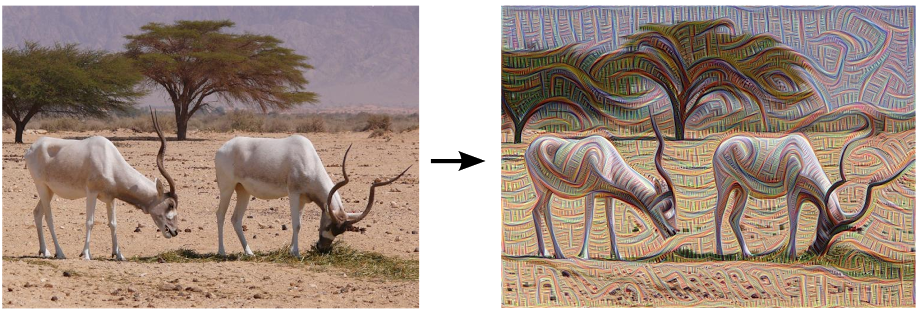
\includegraphics[width=1.0\textwidth]{deep-dream-example}
		\caption{An image before and after processing by Google DeepDream}
	\end{figure}
	
	One of the most recent well-known cases of this is Google's ``DeepDream,'' an online application that uses computer vision technology to enhance images according to detected features, morphing details to exaggerate falsely perceived visual elements (quite commonly biological) resulting in a highly surreal output reminiscent of dreams or hallucinations. This has received popular attention as potentially a form of true AI-created art, with numerous articles discussing the philosophical consideration that it could be considered true art \cite{rayner2016google,galperina2015google} and an actual art exhibition featuring its work \cite{campbell2016inside}.
	
	AI has also demonstrated a surprisingly high proficiency in writing both fiction and non-fiction. Technically-oriented AI writers have already been employed in a professional environment by the company Narrative Science, in the form of their Quill platform: a service that analyses data, identifies data trends and other kinds of useful information, and performs natural language communication to relay results and answer questions \cite{woodie2016big}. Creative AI has also seen recent success as an algorithmically co-written story was recently entered into a literary competition (intended primarily for humans) and outperformed many of its human competitors \cite{tarantola2016ai}. In this sense, computer-human collaboration has already reached the level of a skilled human within the domain of writing. 
	
	\section{Project Aims}
	\label{sec:project-aims}
	
	The aim of this research project is to attempt to bridge some of the gap between the current theoretical state of algorithmic composition and the practical reality of AI in music. The final goal is the development of an algorithm that provides useful melodic material based on the work of a human composer in a manner that is realistically applicable to human composition.
	
	To be considered successful, this algorithm must demonstrate the ability to generate melodic music in a style that is similar to that of an existing musical piece. As the goal in this case is not to simply create a complete song independently but to assist a human in the creation of their own song, the algorithm should not operate fully autonomously. Instead, the algorithm must be able to take musical input from the user and attempt to build on that input in some way. Possible functions to increase gain to the user, such as allowing the user to direct the algorithm's composing via some interactive means are also being searched for. Finally, the program must be be such that its use is feasible in a typical modern compositional context: there must be no hardware, time, or manpower requirements that would be extraordinary for a single musician working independently.
	
	To summarise, the specific objectives of this project are:
	\begin{enumerate}
		\item Survey literature relating to algorithmic melody composition to determine a set of viable methods for expanding existing musical scores
		\item Adapt one or more of these algorithms to write partial melodic sequences that build on and provide variations to an existing melody
		\item Implement an application using this algorithm that allows operation by a non-technical user in a timespan appropriate for practical use (a reasonable estimation would be 1 minute per bar)
		\item Assess the effectiveness of the algorithm(s) in the context of completing a melody through a set of objective tests
		\item Determine, for each algorithm being tested, a strategy that enables user interaction with the melodic generation process in some guiding capacity
		\item Assess the effectiveness of the extended algorithm(s) in the same manner as the original and determine the improvements offered by increased levels of human-computer interaction
	\end{enumerate}
	
	% -----------------------------------------------------------------------------
	
	\chapter{Technical Background}
	\label{chap:technical}
	
	This chapter covers previous work and prominent technology in the field of algorithmic composition, both as a broad overview of the landscape and an in-depth explanation of the particular work directly relevant to this research.
	
	\section{The MIDI Standard}
	\label{sec:midi}
	
	The MIDI (Musical Instrument Digital Interface) standard was published in 1983 as a universal interface for synthesizers  \cite{swift1997brief}. The design of MIDI was such that the format could provide full musical control over any synthesizer device, and enabled communication between any pair of MIDI-enabled devices. The upshot of this was that the MIDI format served as a new kind of compositional notation that could be read and played automatically by any synthesizer device. This later came to include computers with the invention of software synthesizers (discussed in \ref{sec:tech-in-music}), ultimately enabling the use of the PC as a full composer's studio, with the ability to write music with any number of different instruments and have it played back live. 
	% TODO: Expand these two sections, and fix up the accuracy and wording; you can talk more about the specifics of what they do and also make sure stuff is really correct/not misleading
	The MIDI standard is used in most software that deals with music (as opposed to specifically audio), such as DAWs. It is especially useful for algorithmic composition, as it provides a machine-readable format that supports any kind of music with a rich selection of supporting libraries and applications. From an application perspective it is easy to read, write, and play back MIDI files, removing the need to rely on any external application to generate and display a composition. 
	
	% TODO: Clean this up, make it clearer
	The format used by MIDI files is event-based, meaning that every element of a piece of music is recorded as an event happening at some point in time. Time in MIDI files is represented by using a measure called ``ticks,'' whose duration can be set but is typically (and by default) 192 ticks per musical beat, whose duration varies with tempo. Examples of events include note start, note stop, tempo change, instrument change, and repeat section. Each event has a number of parameters, one of which is the type, one of which is the time in ticks as measured from the last event in the track, and the rest of which are usually type-specific (such as pitch or tempo values). Furthermore each MIDI file can contain several tracks, each with their own separate sets of events; these typically represent a single instrument each although each track can play many notes at once. 
	
	\section{Abstract Methods for Algorithmic Composition}
	\label{sec:abstract-methods}
	
	%TODO: You really need to figure out what you're doing with this section mang
	Many common types of AI techniques have been used in some way for algorithmic composition. The majority of these techniques can be broadly categorised as one of:
	\begin{itemize}
		\item Knowledge-based models
		\item Supervised learning
		\item Evolutionary algorithms
		\item Hybrid models
	\end{itemize}
	Each one of these categories carries its own set of advantages and disadvantages which greatly influence the properties of the output it produces. Although techniques from each of these categories can be used for almost any kind of compositional task, different techniques may result in completely different behaviour from the resulting AI. In particular there is a great diversity in the type of input used by algorithms to generate music, which has a large impact on their usability for certain tasks. 
	
	\subsection{Knowledge-Based Models}
	\label{sec:knowledge-systems}
	
	Knowledge-based models use explicitly stored knowledge of some variety to perform computation. They are one of the more intuitive and easy-to-use types of AI, and represent the vast majority of early digital methods for algorithmic composition. There are generally two ways in which this knowledge is obtained; either it is explicitly added by the programmer when the AI is created, or it is learned implicitly from a set of sample cases. The former case has the clear weakness that it can only produce music that it has been explicitly taught how to produce; this puts a harsh limit on the versatility and creativity of the AI. Nonetheless this can be quite an appealing method to use, due to both its computational simplicity and the fact that it can be directly inscribed with compositional principles derived from well-established music theory. Implicitly obtained knowledge on the other hand is much more versatile but is heavily reliant on the quantity and quality of the data provided. The extraction of knowledge from a training set is also a difficult task with many possible solutions - this may also be validly categorised as supervised learning, but is listed here for simplicity's sake. 
	
	%TODO: Find citations for your broad statements, e.g. popularity
	One of the main types of knowledge used in knowledge-based systems is a set of rules/constraints, which is combined with an algorithm that produces an output satisfying these constraints. These techniques are attractive as they have the most direct analogue to music theory. Due to their heavily restricted form however, they are typically poorly suited to performing pure composition. Instead they are typically focused on broad but well-constrained tasks such as harmonization \cite{thomas1985vivace} or jazz improvisation over existing melodies \cite{horowitz1995representing}. Notably in recent decades there has been a significant shift from the use of hard satisfaction of constraints to probabilistic and optimizing methods.
	
	Another common way to store knowledge is as a formal grammar. A formal grammar defines a kind of formal language consisting of a set of symbols that may be arranged according to strict hierarchical structural rules. By creating a grammar that uses musical elements of some kind as its basic symbols, the set of rules used by the grammar can be used to model a style of composition. This is useful when applied to music, due to the natural geometric structure behind most musical composition. However it can also be noted that formal grammars are limited in the degree to which they can comprehend long-term context, an important feature of music that formal grammars struggle to address \cite{moorer1972music}.	 
	
	%TODO: Definitely do this more in-depth, ANNs merit plenty of explanation (and so do HMMs to an extent)
	\subsection{Supervised Learning}
	\label{sec:supervised-learning}
	
	Supervised learning is a subset of machine learning, in which the learning model is trained to approximate some function using a set of clearly defined example inputs and outputs. It is generally applied for tasks involving large-scale data analysis of some kind, such as classifying data samples or identifying relationships between variables in a dataset. It can also be applied to fairly complex decision-based tasks however, as in the case of algorithmic composition. Generally speaking, most supervised learning techniques used for algorithmic composition attempt to model music as a sequential pattern of notes, each associated with some corresponding output depending on the task (such as the subsequent note in melody composition or a harmony in harmonization). This can be considered a specific form of pattern prediction; by understanding the relationship between each set of notes played in a song, you can predict new notes based on a given piece. Due to the popularity and effectiveness of supervised learning in general, it is one of the more popular methods for algorithmic composition. There are two particular classes of supervised learning techniques that are frequently used in algorithmic composition that will be covered here.
	
	\subsubsection{Artificial Neural Networks}
	
	Artificial neural networks (ANNs) are a supervised learning technique that attempt to emulate the actions of neurons within the human brain, useful for their ability to learn arbitrary mappings from one domain to another. This is very useful for composition as network designs can easily be adapted to different compositional tasks or combined with another techniques (see \ref{sec:hybrid-systems}). The majority of ANNs used in music are recurrent neural networks (RNNs), which have a form of ``memory'' allowing them to model sequences of inputs and understand context. Because of this RNNs are powerful tools for composing short melodies and harmonization. They do however still largely fall short at understanding long-term context and at forming coherent song structure. Additionally as in most ML algorithms, the performance of an ANN is heavily dependent on the musical representation used. Because the inputs to a network are strings of numerical (typically binary) values, the music must be translated into an appropriate format, which the ANN must then learn features from. Because of this a representation in which important features are distinctly visible will heavily outperform one in which those features are more obscured.
	
	\subsubsection{Markov Models}
	\label{sec:markov-models}
		
	The other major class in supervised learning are Markov models. A Markov model is a model representing a stochastic process which transitions through a set of states, where the transition probability is dependent only on the current state (i.e. there is no context or memory). The simplest of these is the Markov chain, which simply acts as a state machine where each state emits a fixed output when arrived at and then probabilistically transitions to another based only on the current state. At first glance this appears to be a crippling weakness, as music is intrinsically involves building on a history of musical events; there are a few ways in which this is resolved. Such methods include \textit{n}-order Markov chains, which have memory of the previous \textit{n} states, or the combination of a Markov chain with other processes. These methods have a limited effectiveness, but still display some stark idiosyncrasies that feel ``out of place'' in a melody. More commonly in recent years however is the use of the hidden Markov model (HMM), in which the exact state of the model at any given time is unknown, and each state outputs values with a certain probability. Training this model involves optimizing both the transition and output probabilities to fit the entire length of the training set, resulting in a much more sophisticated overall model. As a result HMMs see much more use in composition, primarily in non-melodic tasks such as harmonization or rhythm.
	
%	\subsection{Evolutionary Algorithms}
%	\label{sec:evolutionary-algorithms}
%	
%	Evolutionary algorithms (EAs) are a relatively recent addition to the algorithmic composition landscape, with the first cases appearing in the early 90s but the majority of practical attempts being made post-2000. EAs are an interesting class of problem solver in that they do not directly solve the problems they are applied to, but instead are a kind of optimization algorithm. One of the keys to an EA is the fitness function it is given; the goal of the EA is to find an optimal input for this function. In the context of music, defining a good fitness function is in itself a very difficult challenge - doing so would mean being able to objectively determine the quality of a musical piece, which is already a major component of the problem of algorithmic composition. Because of this it is quite common to combine EAs with other techniques for use as a fitness function in some capacity. Two of the most common examples of this are training ANNs to act as fitness functions on 
%	
%	% TODO Plenty of stuff to fill in here
%	
%	\subsection{Hybrid Systems}
%	\label{sec:hybrid-systems}

	\section{Artificial Neural Networks}
	\label{sec:ann-overview}
	
	Artificial neural networks (ANNs) are a type of supervised learning model that attempt to emulate the behaviour of networks of neurons within the human brain, and are useful for their ability to learn approximations to functions that are difficult to model directly, particularly ones with large, complex inputs. As a result they are commonly used for challenging learning tasks such as pattern and sequence recognition or automated trading. This property naturally lends itself well to algorithmic composition, a problem that is well-established as being incredibly complex, and for which direct computation has proven largely unsuccessful. 
	
	\subsection{Network Topology}
	
	In essence an ANN is a form of graph consisting of several ordered collections of nodes, called ``layers,'' and weighted directed edges between these nodes from one layer to the next, called ``connections.'' The network operates by activations: Each time the network is activated a set of input values are fed into the network through the first layer, called the input layer, by sending each input value to a corresponding input node. These values propagate from each layer in the network to the next; each node sums the inputs it receives, calculates some function (commonly the standard logistic sigmoid function) of the sum, and propagates this value along all of its outbound connections, multiplying by the connection weight. This propagation continues through the network until it has reached the final layer, called the output layer, which is then read to find the output of the network.
	
	\begin{figure}[!ht]
		\centering
		\begin{tikzpicture}[
		plain/.style={
			draw=none,
			fill=none,
		},
		dot/.style={draw,shape=circle,minimum size=3pt,inner sep=0,fill=black
		},
		net/.style={
			matrix of nodes,
			nodes={
				draw,
				circle,
				inner sep=10pt
			},
			nodes in empty cells,
			column sep=2cm,
			row sep=-9pt
		},
		>=latex
		]
		\matrix[net] (mat)
		{
			|[plain]| \parbox{1.3cm}{\centering Input\\layer} & |[plain]| \parbox{1.3cm}{\centering Hidden\\layer} & |[plain]| \parbox{1.3cm}{\centering Output\\layer} \\
			|[plain]| & & |[plain]| \\
			& |[plain]| & \\
			|[plain]| & & |[plain]| \\
			& |[plain]| & |[plain]| \\
			|[plain]| & & \\
			& |[plain]| & |[plain]| \\
			|[plain]| & & |[plain]| \\
			& |[plain]| & \\
			|[plain]| & & |[plain]| \\
		};
		%Input arrows
		\foreach \ai [count=\mi ]in {3,5,7,9}
			\draw[<-] (mat-\ai-1) -- node[above] {Input \mi} +(-2cm,0);
		% Input -> Hidden
		\foreach \ai in {3,5,7,9}
			{\foreach \aii in {2,4,6,8,10}
				\draw[->] (mat-\ai-1) -- (mat-\aii-2);
			}
		% Hidden -> Output
		\foreach \ai in {2,4,6,8,10}
			{\foreach \aii in {3,6,9}
				\draw[->] (mat-\ai-2) -- (mat-\aii-3);
			}
		% Output arrows
		\foreach \ai [count=\mi ]in {3,6,9}
			\draw[->] (mat-\ai-3) -- node[above] {Output \mi} +(2cm,0);
		\end{tikzpicture}
		\caption{An example feedforward (non-recurrent) ANN}
	\end{figure}
	
	One particular variation of the typical ANN topology that holds a great deal of significance is the recurrent neural network (RNN). This type of network contains recurrent connections that are directed backwards through the network layers (or from a layer to itself). These connections do not propagate values during an activation in the same way as ordinary connections, but instead carry the values through to the next activation; this effectively gives the network a form of memory, as the receiving nodes receive inputs from the previous activation. There are many possible ANN constructions, such as Adaptive Resonance Theory networks which contain two layers fully connected to each other and are used for recognition or prediction tasks, but in this paper only simple RNNs will be discussed.
	
	\subsection{Training}
	
	As with any supervised learning model, ANNs must be trained on a dataset in order to be useful. In the case of ANNs specifically, each dataset used for training is composed of a set of inputs and corresponding outputs, which map to the input and output layers of the ANN respectively. The actual act of training an ANN is performed by adjusting the weights of the connections in the ANN so that the input values of the dataset are approximately mapped to the correct output when activating the ANN. One of the most common ways of achieving this is a technique called ``backward propagation of errors,'' or backpropagation.
	
	The backpropagation algorithm is a form of optimization method, where the objective is to minimize the output error of the ANN being trained. This error is calculated by activating the ANN with a test input, then calculating the difference between the ANN's output and the correct output as a derivative of the connection weights in the network. These error values are then used to adjust the weights of the connections via gradient descent (or some similar method). This is repeated for a number of epochs, with the ANN moving towards a more accurate model of the target function each time. As with most optimization-based learning algorithms, this process is vulnerable to becoming stuck in local minima. It can therefore be effective in certain cases to retrain a network several times and select the best performing as the final model.
	
	\section{Markov Models}
	
	Markov models are another class of supervised learning method, which attempt to model sequential data as a stateful stochastic process without memory. Although there are several different types of specific models based on this method, they can all be described by a set of states and probabilistic transition functions between these states; typically this is represented by some form of directed graph. Markov models are often used to model probabilistic processes in which all the relevant information of the system can be captured in a single pre-defined state. Different types of Markov model are applicable to quite different tasks owing to their special properties; for example, Markov chains are useful for modelling certain natural processes, particularly in physics or chemistry simulations, while partially observable Markov decision processes (POMDPs) are useful for problems such as automated robot navigation.
	
	\subsection{Markov Chains}
	
	Markov chains are a type of Markov model in which each state is directly observed as an output of the system being modelled, and the transitions between these states are stochastic and autonomous, meaning that they occur with a certain probability that is not influenced by any input to the system. Algorithms based on Markov chains were some of the first learning models applied to music, with one of the first academic examples appearing as early as 1961 \cite{olson1961aid}. The main appeal of Markov chains in this field is that they are a simple but powerful way to model data that is highly sequential, which strongly applies to music. There have been a wide variety of methods for using Markov chains in composition, as they are fairly basic and so can be integrated into many different systems; some examples of this include using Markov chains trained on classical music as fitness functions for an evolutionary algorithm \cite{lo2006evolving}, or generating a basic melodic pattern with Markov chains and then refining it using an ANN \cite{verbeurgt2004hybrid}. 
	
	\subsection{Hidden Markov model}
	
	Hidden Markov models (HMMs) are a type of Markov model in which the state transitions are autonomous (i.e. there is no input) but the actual state at any given time is ``hidden.'' This means that the states of the HMM cannot be directly observed, but only inferred (probabilistically) based on the visible output that they emit. This is useful for modelling any kind of sequential data which can only be observed via a dependent sequential variable; examples include complex processes such as cryptanalysis, language translation, or protein folding. A notable advantage that HMMs have over Markov chains is that they are able to learn features that are not necessarily immediately reflected in the output data; this gives them an advantage in algorithmic composition, as they are able to learn a limited form of context for notes.
	
	\section{Artificial Neural Networks in Algorithmic Composition}
	\label{sec:anns}
	
	As described in section \ref{sec:ann-overview}, artificial neural networks (ANNs) are a powerful class of techniques for approximating functions, and recurrent neural networks (RNNs) extend their functionality to add a form of memory allowing for the comprehension of sequential data. Within this class there have been many different techniques created for performing melodic composition, with many featuring unusual novelties and useful unique properties.
	
	\subsection{Jordan Network With Sparse Pitch Representation and Planning Units}
	\label{sec:todd-net}
	
	The first well-documented attempt at using ANNs for musical composition was made by Peter Todd \cite{todd1989connectionist}, who created a simple 3-layered RNN with a topology based on a Jordan network \cite{jordan1997serial} which composed monophonic melodies.
	
	The representation of musical data used by the network is quite basic and has limited scope. The temporal dimension of a song is represented by dividing it into a set of discrete timesteps at fixed intervals, and at each of these timesteps exactly 1 note may be played or sustained. The input string to the network represents 1 timestep, and consists of a set of values representing pitches, 1 value representing the start of a new note, and a set of values corresponding to ``plans.'' The pitch value for a given timestep is represented simply by taking the pitch of the note $p$ within some user-defined scale (Todd used the C major scale with $p = 0$ for D4 up to $p = 14$ for C6), then setting the $p$-th pitch input to 1 and all others to 0. This only allows a fairly limited range of notes to be played, which reduces the versatility of the network. The value of the ``new note'' input is 1 if a note was started during the timestep, and 0 otherwise. Finally, the ``plan'' inputs have their values set according to the song; each song has a corresponding set of plan inputs, which are fixed throughout processing, and may or may not overlap with other the ``plans'' of other songs. This input is used by the network to differentiate between the songs that it is trained with, allowing it to behave differently depending on the intended output. Finally, the output of the network is of the same format as the input sans the plan units, and represents the network's estimate for the next timestep.
	
	This particular type of Jordan network is similar to a basic feed forward ANN, with an input layer, a hidden layer, and an output layer, with the input and hidden layers fully connected to the layer ahead. In addition to these connections, two recurrent connections are added: a connection from each $i$-th output neuron to the $i$-th input neuron with weight 1, and a connection from each input neuron to itself (with the exception of the plan neurons) with weight $\alpha < 1.0$ (Todd used $\alpha = 0.7$). This effectively treats the network's output as its input for the next iteration, and causes its inputs to slowly decay instead of disappearing with each iteration. This gives the network an effective memory of recent notes that have been played, with each pitch fading out of memory the longer it goes without being played.
	
	\begin{figure}[!ht]
		\centering
		\begin{tikzpicture}[
		plain/.style={
			draw=none,
			fill=none,
		},
		dot/.style={draw,shape=circle,minimum size=3pt,inner sep=0,fill=black
		},
		net/.style={
			matrix of nodes,
			nodes={
				draw,
				circle,
				inner sep=10pt
			},
			nodes in empty cells,
			column sep=2cm,
			row sep=-9pt
		},
		>=latex
		]
		\matrix[net] (mat)
		{
			|[plain]| \parbox{1.3cm}{\centering Input\\layer} & |[plain]| \parbox{1.3cm}{\centering Hidden\\layer} & |[plain]| \parbox{1.3cm}{\centering Output\\layer} \\
			& |[plain]| & \\
			|[plain]| & \\
			& |[plain]| & \\
			|[dot]| & & |[dot]| \\
			|[dot]| & |[plain]| & |[dot]| \\
			|[dot]| & & |[dot]| \\
			& |[plain]| & \\
			|[plain]| & \\
			& |[plain]| & \\
			|[plain]| & & |[plain]| \\
			& |[plain]| & |[plain]| \\
			|[plain]| & & |[plain]| \\
			& |[dot]| & |[plain]| \\
			|[dot]| & |[dot]| & |[plain]|\\
			|[dot]| & |[dot]| & |[plain]| \\
			|[dot]| & \\
			& |[plain]| & |[plain]| \\
		};
		%Input arrows
		\foreach \ai [count=\mi ]in {2,4}
			\draw[<-] (mat-\ai-1) -- node[above] {Pitch \mi} +(-2cm,0);
		\draw[<-] (mat-8-1) -- node[above] {Pitch $p$} +(-2cm,0);
		\foreach \ai [count=\mi ]in {12,14}
			\draw[<-] (mat-\ai-1) -- node[above] {Plan \mi} +(-2cm,0);
		\draw[<-] (mat-18-1) -- node[above] {Plan $n$} +(-2cm,0);
		\foreach \ai [count=\mi ]in {10}
			\draw[<-] (mat-\ai-1) -- node[above] {New Note} +(-2cm,0);
		% Input -> Hidden
		\foreach \ai in {2,4,8,10,12,14,18}
			{\foreach \aii in {3,5,7,9,11,13,17}
				\draw[->] (mat-\ai-1) -- (mat-\aii-2);
			}
		% Input -> Input
		\foreach \ai in {2,4,8,10}
			{\foreach \aii in {3,6,9}
				\draw[->,line width=0.3mm] (mat-\ai-1) edge[loop right] (mat-\aii-2);
			}
		% Hidden -> Output
		\foreach \ai in {3,5,7,9,11,13,17}
			{\foreach \aii in {2,4,8,10}
				\draw[->] (mat-\ai-2) -- (mat-\aii-3);
			}
		% Output arrows
		\foreach \ai [count=\mi ]in {2,4}
			\draw[->] (mat-\ai-3) -- node[above] {Pitch \mi} +(2cm,0);
		\draw[->] (mat-8-3) -- node[above] {Pitch $p$} +(2cm,0);
		\draw[->] (mat-10-3) -- node[above] {New Note} +(2cm,0);
		% Output -> Input
		\foreach \ai in {2,4,8,10}
			\draw[->,line width=0.4mm] (mat-\ai-3) edge[bend left] (mat-\ai-1);
		\end{tikzpicture}
		\caption{The topology of Todd's network, with recurrent connections bolded}
	\end{figure}
	
	The network is trained using standard backward propagation of errors with gradient descent. The training data is extracted from a set of songs by converting each song to the timestep format as described above, and providing them as input to the network. It is important to note that in traditional operation of the network, the only input to the input layer comes from the recurrent connections from the input layer and the output layer. However this leads to decreased performance during training, due to the fact that the input layer is receiving values from the output layer that are different to the expected output at that stage. Put simply, this means that instead of learning to map each timestep in the training song to the following timestep, the network learns to map the output from its current untrained state to the following timestep in the original song. This problem disappears as the network begins to converge and its actual output begins to match the expected output, but this can take a great deal of time as the training process is essentially chasing a moving target - the network is repeatedly trained to learn an incorrect mapping until it has converged enough to start learning the correct mapping. To overcome this problem, the training process eschews the recurrent connection from the output to input layers and instead directly provides the timesteps from the training song as input, allowing the network to start learning the ``real'' mapping immediately.
	
	This network was found to perform reasonably well by Todd. The primary testing metric used in the original paper was the computation required for the network to learn to recreate a number of distinct melodies. The results were fairly promising for the time, with a network of hidden layer size 15 being sufficient to learn up to 4 different songs of 34 time steps each. The number of epochs of training required notably scaled linearly with the number of songs; 2,000 for 1 song, 4,500 for 2 songs, and 8,500 for 4 songs. Reducing the number of hidden units from 15 to 8 however increased the number of epochs required to learn 2 songs to 50,000, due to the increased difficulty of representing the complex patterns of the song with a simpler function.
	
	Following this, a subjective assessment was formed on the ability of the network to create new melodies outside of the training set. This displays one of the advantages of using planning units, as by enabling or disabling different plan inputs the network can be made to output songs of different styles drawing inspiration from one or more of the training songs. A number of observations were made about the original compositions produced by the network: one interesting property it displayed was that when using a single plan unit it tended to output melodies consisting of strings of pitches from the corresponding training melody, but stitched together in new orders at points where the pitches aligned. This ultimately results in the melodies eventually beginning to loop, as at some point the network ends up in a similar state to its initial state and starts playing the opening sequence again. It was also observed to have a very weak understanding of rhythm - the single neuron for representing the start of new notes was insufficiently complex to model the structured nature of musical rhythm. Despite training, the network was unable to recognize a relationship between pitch changes and note beginnings.
	
	\subsection{Elman Network with Circle-of-Thirds Pitch and Chaotic Inspiration}
	\label{sec:coca-net}
	
	An alternative simple RNN to the Jordan network as described above is the Elman network \cite{elman1990finding}. The topology of an Elman network is similar to that of a Jordan network, but with different recurrent connections. While in the Jordan network the recurrent feedback is received in the input layer, in the Elman network it is instead received in the hidden layer. The specific model of Elman network for composition described here is as designed by Coca, Romero, and Zhao \cite{coca2011generation}.
	
	\begin{figure}[!ht]
		\centering
		\begin{tikzpicture}[
		plain/.style={
			draw=none,
			fill=none,
		},
		dot/.style={draw,shape=circle,minimum size=3pt,inner sep=0,fill=black
		},
		net/.style={
			matrix of nodes,
			nodes={
				draw,
				circle,
				inner sep=10pt
			},
			nodes in empty cells,
			column sep=2cm,
			row sep=-9pt
		},
		>=latex
		]
		\matrix[net] (mat)
		{
			|[plain]| \parbox{1.3cm}{\centering Input\\layer} & |[plain]| \parbox{1.3cm}{\centering Hidden\\layer} & |[plain]| \parbox{1.3cm}{\centering Output\\layer} \\
			& |[plain]| & \\
			|[plain]| & \\
			& |[plain]| & \\
			|[dot]| & |[plain]| \\
			|[dot]| & & \\
			|[dot]| & |[plain]| \\
			& |[plain]| & \\
			|[plain]| & \\
			& |[plain]| & \\
			|[plain]| & |[plain]| & |[plain]| \\
			& |[plain]| & \\
			|[plain]| & |[plain]| & |[plain]| \\
			& |[plain]| & \\
			|[plain]| & |[plain]| & |[plain]| \\
			& |[plain]| & \\
%			|[dot]| & |[plain]| & |[plain]| \\
%			|[dot]| & |[plain]| & \\
%			|[dot]| & |[plain]| & |[plain]| \\
%			& |[plain]| & \\
%			|[plain]| & |[plain]| & |[plain]| \\
%			& |[plain]| & \\
%			|[plain]| & |[plain]| & |[plain]| \\
%			& |[plain]| & \\
%			|[dot]| & |[plain]| & |[plain]| \\
%			|[dot]| & |[plain]| & \\
%			|[dot]| & |[plain]| & |[plain]| \\
%			& |[plain]| & |[plain]| \\
		};
		% Input arrows
		\foreach \ai [count=\mi ]in {2,4}
			\draw[<-] (mat-\ai-1) -- node[above] {Pitches \mi} +(-2cm,0);
		\draw[<-] (mat-8-1) -- node[above] {Pitches 7} +(-2cm,0);
		\draw[<-,align=center] (mat-10-1) -- node[above] {Lower \\ Octave} +(-2cm,0);
		\draw[<-,align=center] (mat-12-1) -- node[above] {Higher \\ Octave} +(-2cm,0);
		\foreach \ai [count=\mi ]in {14,16}
			\draw[<-] (mat-\ai-1) -- node[above] {Duration \mi} +(-2cm,0);
		% Input -> Hidden
		\foreach \ai in {2,4,6,8,10}
		{\foreach \aii in {3,6,9}
			\draw[->] (mat-\ai-1) -- (mat-\aii-2);
		}
		% Hidden -> Hidden
		\foreach \ai in {3,6,9}
			\draw[->] (mat-\ai-2) edge[in=150,out=30,loop] (mat-\ai-2);
		% Hidden -> Output
		\foreach \ai in {3,6,9}
		{\foreach \aii in {2,4,6,8,10}
			\draw[->] (mat-\ai-2) -- (mat-\aii-3);
		}
		% Output Arrows
		\foreach \ai [count=\mi ]in {2,4,6,8,10}
		\draw[->] (mat-\ai-3) -- node[above] {Ouput \mi} +(2cm,0);
		\end{tikzpicture}
		\caption{An example of a variety of Elman network}
	\end{figure}
	
	The representation of music used by this particular network is quite different to that used in \ref{sec:todd-net}. Most distinctly it does not use the timestep representation for the temporal dimension, but instead assigns a duration value to each event. This shares the disadvantage of only allowing monophonic input/output, but places a greater emphasis on learning the temporal features of the input data. This helps overcome some of the issues mentioned earlier with regard to the ``new note'' feature. The representation for the duration of a note is given as a binary string whose actual binary value represents the duration of the note. The conversion between numerical value and musical time is such that a crotchet (quarter note) has a duration value of 96. This is the exact value used by the MIDI standard (\ref{sec:midi}), chosen such that it can represent all standard note divisions (semiquavers, crotchet triplets and quaver triplets) as well as the small irregularities in timing that occur during live performance. 
	
	The pitch representation is also quite different, as there is no longer a one-to-one mapping of pitches to nodes. Instead, the pitch is split into two parts: the in-octave pitch and the octave. The representation for the octave is very simple and uses only 2 nodes, with the binary mapping $10 = \text{C2-B2}$, $01 = \text{C4-B4}$, and $00 = \text{C3-B3}$, with the network's output being snapped to the closest of these values. This can easily be extended to cover a wider range with a small increase in nodes, making this representation more versatile than the one used in Todd's design. The representation for the in-octave pitch is also split into two parts, based on intervals of 4 and 3 semitones (major and minor thirds). Each circle represents a set of pitches whose relative intervals are multiples of 4 and 3 for major and minor thirds respectively. A given note is then represented as a pair of binary strings length 3 and 4 representing the index of the circles it lies in. So for example, C is encoded as 1000 100, D is encoded as 0010 001, and E is encoded as 1000 010. This is a useful representation as it models relative pitch (for certain intervals), which is more relevant in most musical structure than absolute pitch, without some of the disadvantages imposed by purely relative pitch representation such as easily straying off-key. 
	
	\begin{figure}[h]
		\centering
		\includegraphics[width=0.8\textwidth]{circles-of-thirds}
		\caption{The circle-of-thirds representation of pitch; the upper row circles contain intervals of major thirds, and the lower row minor thirds. Each pitch within a 12 semitone octave can thus be uniquely identified by a pair of circles.}
	\end{figure}
	
	\subsubsection{Chaotic Inspiration}
	\label{sec:chaotic-inspiration}
	
	The network also features an additional set of input nodes used for chaotic inspiration based on the algorithm described in \cite{coca2010characterizing}. This algorithm is based on the principle of generating music through chaotic dynamical systems. This is a branch of algorithmic composition, first explored in the late 1980s \cite{pressing1988nonlinear}, that differs greatly from the AI methods previously explained; instead of attempting to directly model compositional methods in some way, a mathematical model is developed that maps systems with chaotic behaviour to musical scores. The power of these systems comes from the fact that these models generate fractal objects with structures similar to those found in the analysis of classical music. Naturally most results in this area are not well suited to composing complete musical scores due to their unrefined and somewhat erratic nature, but are quite well suited to producing musical material from which a composer can be inspired.
	
	Coca, Tost, and Zhao's algorithm uses a nonlinear dynamic system consisting of three variables. These variables are drawn from an existing melody, with the first being extracted from pitches, the second from rhythm, and the third from musical dynamics (amplitude and velocity). It also takes a set of inputs defining a specification for the musical scale in which the output piece is to be written. The algorithm then uses these inputs to map the extracted variables into a new melody, stored in the MIDI file format (\ref{sec:midi}). As is expected from a chaotic system, a small change to the input variables can cause a disproportionately large change to the output values while still producing a result of similar quality.
	
	This algorithm is used to generate a source of ``inspiration'' that can be used in the creation of a melody. The goal of inspiration in the context of algorithmic composition is to create variations in the melody generation process by modifying the system in a way that preserves the original information; typically this is accomplished by adding a new input to the system which provides a source of variance. This is very useful for systems in which a large number of possible outputs are desired, such as those that present their results to some selection process (e.g. evolutionary algorithms). The use of chaotic algorithms to generate this inspiration is advantageous due to the fact that their output has a similar fractal structure to real music, meaning that a given inspirational segment contains a structure that the final output melody will be built on in some way.
	
	In this particular compositional algorithm, the input melody from which the chaotic inspiration is drawn is the same as the melody being learned during training, or the melody being recreated while composing. A subset of the notes from the chaotic inspiration are provided as input to the network, fed sequentially to the network cyclically alongside the base melodic input. In the paper (\cite{coca2011generation}) the varied results are provided by changing the number of notes taken from the chaotic inspiration as input.
	
	\section{Distance Modelling with Hidden Markov Models for Monophonic Rhythms}
	\label{sec:distance-model}
	
	As discussed in section \ref{sec:supervised-learning}, Markov models tend to have trouble with the kind of complex structure involved in melodic pitch sequences. Using a hidden Markov model helps improve the model's performance in dealing with more complicated sequential patterns. While this type of model is still quite weak in terms of comprehending pitch, it is more capable of recording and recreating simple rhythmic patterns across moderate durations. While this alone is not a common use for HMMs due to their inability to model true long-term patterns, they can be used as part of a hybrid system using a model of rhythmic distances to greater effect \cite{paiement2007generative}.
	
	\subsubsection{Hidden Markov Model}
	
	The HMM used to model rhythmic patterns uses a fairly straightforward timestep representation for monophonic rhythm. A melody is divided up into fixed time intervals, similarly to the representation in \ref{sec:todd-net}, and at each such timestep a value is given: 0 if no note is playing during the timestep, 1 if a note was started, and 2 if a note is being sustained. The melody's rhythm is then represented by an array in which the \textit{n}-th element corresponds to the \textit{n}-th timestep.
	
	The HMM can then be trained on this system by treating the array as a sequential dataset. The HMM is taken to have multinomial (discrete) emission values $\{0,1,2\}$, and is fitted to the given dataset using Expectation-Maximization. This results in a model that generates rhythm stochastically, with an expected outcome equal to the training rhythm. The particular behaviour of the HMM is quite useful for generating rhythm, as it tends to learn very well what note lengths are common/acceptable and which note lengths are more or less likely to follow others. The main weakness that it displays however is the inability to adapt to the long-term rhythmic structure of a song; although short patterns are within its grasp the stochastic nature of the HMM prevents it from recalling features such as the repetition of a pattern every 4 bars. 
	
	\subsubsection{Distance Model}
	
	To overcome this drawback the HMM can be combined with a suitable long-term rhythm model; in this case, rhythmic distance between fixed rhythmic partitions is used. The representation used is the same as with the HMM as described above, and the distance measure between each pair of partitions is their Hamming distance. The most natural way to divide up a rhythm is by bars/measures, as these are the units of time upon which the structure of a melody is fundamentally built. It is also possible however to use many different partitions as part of the same model - although using divisions smaller than a bar is not recommended in most cases, using many consecutive bars can give useful results when dealing with certain long-term patterns, such as a repeating 4 bar pattern.
	
	%TODO: Basically this shit is pretty dense in the original paper; you're gonna have to unfuck their explanation somewhat because otherwise it will probably not be understood
	
	The distance model operates by learning a distribution of possible distances between each pair of partitions within the training melodies according to distance constraints. The constraints between partitions $i$ and $j$ (for $i<j$) within a melody are given by:
	\begin{equation*}
		\begin{split}
		\alpha_{i,j} &= \min_{k \in \{1,\dots,(i-1)\}} (d_{k,j} + d_{i,k}) \text{ and} \\
		\beta_{i,j} &= \max_{k \in \{1,\dots,(i-1)\}} (|d_{k,j} - d_{i,k}|),
		\end{split}
	\end{equation*}
	where $d_{i,j}$ is the Hamming distance between partitions $i$ and $j$. It follows by the triangle inequality that:
	$$\beta_{i,j} \leq d_{i,j} \leq \alpha_{i,j} \text{ .}$$
	From this, the distribution of possible distance values between any pair of partitions can be calculated as dependent on the distributions of $\alpha_{i,j}$ and $\beta_{i,j}$. Specifically, the variable $d_{i,j} - \beta_{i,j}$ is modelled by the binomial distribution:
	$$B(\delta, \alpha_{i,j}, \beta_{i,j}, p_{i,j}) = \binom{\alpha_{i,j} - \beta_{i,j}}{\delta} p_{i,j}^\delta (1-p_{i,j})^{\alpha_{i,j}-\beta_{i,j}-\delta} \text{ ,}$$
	where $\beta_{i,j} + \delta = d_{i,j}$ and $p_{i,j}$ is the probability a pair of symbols from partitions $i$ and $j$ differ. 
	
	That this model is accurate depends on the random variable $(d_{i,j}-\beta_{i,j})/(\alpha_{i,j}-\beta_{i,j})$ being identically distributed among each song in the training set. For obvious reasons this is not in itself a safe assumption to make; however it is very common for certain rhythmic patterns to recur within genres and styles of music, e.g. verses in pop music using the same rhythm in every phrase, or rock drums repeating the same pattern each bar except for the end of every four bars. Therefore instead of using a simple binomial distribution, a binomial mixture distribution is employed, in which each subpopulation is given by a set of songs that have similar rhythmic features. This binomial mixture model can then be learned through Expectation-Maximization \cite{bilmes1998gentle}, clustering the training set into subpopulations according to values of $(d_{i,j}-\beta_{i,j})/(\alpha_{i,j}-\beta_{i,j})$ in order to obtain the initial parameter estimate for the mixture model.
	
	From this model, a probability distribution for the distance between a partition and each prior partition can be calculated. After determining $\beta_{i,j}$ and $\alpha_{i,j}$, whose values are not dependent on $d_{i,j}$, the probability $p(d_{i,j})$ can be given by:
	$$p(d_{i,j} = \beta_{i,j} + \delta) = \sum_{k=1}^{c} w_{i,j}^{(k)} B(\delta,\alpha_{i,j},\beta_{i,j},p_{i,j}^{(k)}) \text{ ,}$$
	where $c$ is the number of subpopulations, $p_{i,j}^{(k)}$ is the value of $p_{i,j}$ learned for the $k$-th subpopulation, and $w_{i,j}^{(k)}$ is the size of the $k$-th subpopulation (normalized so that $\sum_{k=1}^{c} w_{i,j}^{(k)} = 1$). The total probability for the rhythm of partition $j$ may then be calculated as $\prod_{i=1}^{j-1} p(d_{i,j})$. If using multiple partition divisions, the probabilities calculated for each division type are multiplied to find the overall probability. 
	
	\subsubsection{Combined Model}
	
	As the distance model does not at all cover short-term rhythmic structure, it is natural to combine it with a model that does, i.e. the rhythmic HMM discussed above. This combination also useful as a way to traverse the search space, as the distance model is not generative - it defines probability values for rhythms in partitions but does not have an efficient way to search the space of possible rhythms (size $3^l$, where $l$ is the number of timesteps per partition) for an optimal value. The use of an HMM in a generative capacity resolves this issue.
	
	The algorithm to create a partition of rhythm with these two models is comparatively simple. First the HMM generates a rhythm of the appropriate length, $\{x_1,\dots,x_l\}$. Then for each index $j$ in the rhythm array, the value at that index $x_j$ is set as:
	$$ x_j = \argmax_{a \in \{0,1,2\}} \left[ \log p_{HMM}(\mathbf{x^*} | \{y_1,\dots,y_m\}) + \lambda \log p_{DIST}(\{y_1,\dots,y_m,\mathbf{x^*}\}) \right] \text{ ,}$$
	where $\{y_1,\dots,y_m\}$ is the melody preceding the new partition, $p_{HMM}(x)$ and $p_{DIST}(x)$ are the probabilities of $x$ according to the HMM and distance model respectively, $\lambda$ is a constant (explained further below), and $\mathbf{x^*} = \{x_1,\dots,x_{j-1},a,x_{j+1},\dots,x_l\}$.
	
	This process repeats until it the partition reaches a stable value, i.e. none of $x_1$ to $x_l$ change during an iteration. The objective of this algorithm is to find a solution that tried to maximize likelihood according to both of the models. Specifically, this algorithm is a form of the Greedy Max Cut method \cite{rohde2002methods}, a Multidimensional Scaling optimization algorithm which has proven to be optimal in terms of running time and performance for this type of search problem. Of particular importance is the constant $\lambda$, which sets a balance between the two constraints being optimized; high values of $\lambda$ prioritize the distance measure, while low values prioritize the HMM.
	
	
	
	\chapter{Project Execution}
	\label{chap:execution}
	
	In this chapter the requirements and objectives of the algorithm being sought are covered, and an in-depth design of the algorithms chosen is presented along with the details of their implementation.
	
	\section{Design}
	
	The algorithm being selected and adapted for this project is intended to fulfil the goals discussed in \ref{sec:project-aims}, but these stated aims leave a huge degree of room for the implementational details of the algorithm. As touched on in section \ref{sec:abstract-methods}, there are many different ways to perform algorithmic composition, and the ``ideal'' method is entirely dependent on the exact requirements of the user. In this section these requirements are detailed and a pair of algorithms that satisfy them are given. 
	
	\subsection{Requirements and Objectives}
	
	To briefly recap the aims in \ref{sec:project-aims}, the algorithm was to be designed such that it is able to build on existing melodic material in a way that is both musically sound and consistent with the material's style. This is a fairly open-ended task that can be fulfilled in many different ways by many different means. Given the scope of this project it was therefore important that the limits of this algorithm be well-defined from the outset. Some of the factors that needed to be taken into consideration when defining these limits were the melodic properties (e.g. harmonies, long-term song structure, rhythmic micro-variations) recognized by the algorithm, the hardware and data requirements, and the execution time of the melody generation process. 
	
	One of the most significant limitations to the algorithm's design was the number of simultaneous musical elements it would be able to process, i.e. monophonic or polyphonic melody and the use of multiple instruments within a melody. It is easy to see that allowing for more notes and voices to be played at the same would increase the complexity of the algorithm to a large degree; exactly to what extent depends on the details of the algorithm. Some methods are easily adapted or are fundamentally built around the concept of simultaneous notes \cite{boenn2008automatic}, while others use musical representations that would need to be completely overhauled to enable polyphony \cite{todd1989connectionist}. While polyphonic melody construction and harmonization play major roles in composition, they add a degree of complexity to the output that would greatly increase the difficulty of achieving a suitable result within this research, both due to algorithmic complexity and a significant increase in the difficulty of testing. The same applies to the inclusion of multiple instruments - especially if the algorithm is to understand the difference between their sounds in relation to music. Because of this, the algorithm was designed to read and write only single-voiced monophonic melodies. 
	
	The other major feature that needed to be considered for the algorithm's design was its ability to recognize long-term features of a melody. This includes recurring motifs, common rhythm patterns, repeating variations of phrases, and recognizing sections such as the verse and chorus. Being able to recognize and predict these features is a weakness of most compositional AI, as the relationships between distant measures are often quite complex and can be difficult to model computationally, although some attempts have been made to specifically target this problem \cite{tokui2000music,paiement2007generative}. This particular algorithm exists in an interesting position with regard to this situation: Input from the user can be used to label these features, making it much easier for the algorithm to use them; but as the algorithm merely produces material for the user to create a song with, it is simultaneously less important that the algorithm actually focus on long-term features. As a result, the decision of how much the algorithm should try to capture long-term structure was a balance between utility to a potential user and the additional effort required by the user to operate this feature. Ultimately it was determined that putting a great deal of emphasis on true long-term features would be mostly useless for the algorithm, as there is no desire for it to actually arrange songs from such a high level; while such an algorithm might be useful for composers in some contexts, it is quite tangential to the particular goals of this research. Instead the algorithm should only attempt to learn features over shorter periods of several measures or phrases, giving it suitable context to produce human-like material in most circumstances while not requiring a significantly more complex design or degree of user interaction. 
	
	Beyond the algorithm's pure ability to model music, there are additional constraints posed by the problem. The most obvious of these is time, a particularly sensitive aspect as the AI is intended to be used by individuals as a tool for creative work. While the algorithm presented in this work is not intended to be a finished product suitable for practical use, if it fundamentally has a high asymptotic time complexity then it may never be useful in any real scenario. Another important factor is the reliance of the algorithm on data. This is notably only a factor at all for supervised learning techniques, but it is particularly discouraging in the case of music as useful musical data (such as well-formatted MIDI songs) can be hard to obtain (see \ref{sec:midi-data}). Finally the algorithm should feature some degree of non-determinism. The reason for this is that there is virtually no way to guarantee that the algorithm's output is useful to the user; even if it can be considered musically sound in all senses and fits perfectly into the original melody, it may simply not be to the user's liking. It is therefore necessary that the user can view a range of material to be inspired from, to maximize the algorithm's possible utility.

	Additional features such as modelling human-like imperfections in performance or musical dynamics were considered, but deemed to be tertiary to the core goals of the algorithm. This and the above comprised the basic functional requirements for the algorithm. These requirements still leave a great deal 
	open about the algorithm, both in its implementation details and exactly how its success in imitating a style and producing coherent output is measured.

	\subsection{Algorithm Selection}
	\label{sec:algorithm-selection}
	
	One of the most promising avenues from the outset appeared to be evolutionary algorithms, although they did not prove ultimately suitable. The main advantage of EAs in music is that they search the space of possible melodies by assigning a fitness score to each melody that they consider; this is trivially made into a user-driven selection process by allowing the user to assign fitness scores, ensuring that higher quality melodies are successfully selected for. This method has some unfortunate drawbacks however, with the first and foremost being that EAs typically attempt an enormous number of solutions before reaching a passable solution, especially when working in a large domain with many dimensions such as melodies. This results in an unacceptable level of fatigue being inflicted on the user rating the melodies. There have been numerous attempts to overcome this problem, using methods such as clustering similar results to avoid presenting the user with many similar melodies \cite{burton1998hybrid,ralley1995genetic}, or trying to minimize the number of evolutionary iterations \cite{marques2010interactive}. While these methods do show some promise, it is still a substantially difficult task to compose a melody of sufficient quality with a small enough time and interaction count to be appropriate for this task.

	Focusing instead on the user-facing constraints of the problem suggests that the ideal algorithm would be one that performs generation quickly and at most relies on explicit user input to refine suitable results, not as a lynchpin of the generative process. The best candidates for this are the supervised learning techniques previously discussed in section \ref{sec:supervised-learning}, which learn features of melodies from a training corpus and use this model to create new melodies in the same style. This allows for rapid creation of quality work, as the majority of computation is performed prior to the generation step. In particular the two most commonly used learning techniques in algorithmic composition are hidden Markov models and recurrent neural networks. These structures are designed for learning prediction models over sequential data, and can be designed to write new music by predicting the next note at a given point in time. 
	
	There are some trade-offs between a supervised learning approach and a knowledge-based approach. One of the most significant advantages of supervised learning is that it is far more versatile, as it does not require any kind of hand-encoded knowledge. This is vital for an application that is intended as a generic tool for composers, as it must be able to write virtually any style of music - an infeasible goal with an entirely hand-written set of rules. It does however often suffer from an inability to learn long-term patterns very well; the general technique for using supervised learning to compose music is to predict notes as sequential data. This usually gives good results over the short term, but fails to learn relationships between distant patterns. In this particular case however, the presence of the user can mitigate this weakness by providing relevant long term features as input to the algorithm, while the issue of versatility can only be overcome if the user provides a their own set of constraints to write their songs with. Given that one of the goals in this work was to minimize the amount of work on the part of the user, it was a natural decision to user supervised learning. As a point of interest there do exist supervised learning models that learn rules from a corpus of data, potentially satisfying the major issues at hand, but it is an infrequently used technique that has not thus far have been used for melodic composition. 
	
	Given that the focus of the algorithm's design is melodic composition, it was preferable to focus on techniques that specialize in this area; within the realm of supervised learning this would logically imply ANNs (\ref{sec:anns}). Although there exist other suitable techniques, such as rule-learning models (\ref{sec:knowledge-systems}) and HMMs (\ref{sec:markov-models}), uses of these techniques in the literature are generally focused on harmonization and counterpoint tasks rather than monophonic melodic composition. There are many ways to use ANNs for composition, such as a fitness function for some optimizing algorithm \cite{manaris2007corpus} or as part of a constraint architecture \cite{hild1992harmonet}. However ANNs have been chosen here for specific reasons (i.e. fast run-time and versatility) that will be best satisfied by a more pure approach. %TODO Don't forget to give those justifications properly before this point
	
	Of the algorithms that were reviewed, two appeared to be well-suited to the task. These algorithms were both fairly simple implementations of RNNs, each using a relatively basic melody generation algorithm that featured no cumbersome or overly complex architecture. This ensured a good generation speed and a straightforward training process, as well as a high degree of versatility - as is typical for ANNs. The algorithms are detailed below in \ref{sec:implementation}, including references to the base algorithms as well as the modifications introduced within this work.
	
	\section{Musical Data}
	\label{sec:midi-data}
	
	As both of the algorithms implemented here use supervised learning, it was necessary to train them with a set of data. This application is concerned only with the purely melodic aspects composition as opposed to dynamics or timbre, therefore only the musical score is required as input. This requirement is best satisfied by the MIDI format (\ref{sec:midi}), which directly encodes scores. This is also a convenient choice due to the availability of many useful libraries that provide functions for reading, writing, and manipulating MIDI data. 
	
	One unfortunate difficulty involved with using MIDI data, however, is availability. Due to the limited range of sound produced by MIDI synths, such as Microsoft's GS Wavetable SW Synth, it is not a popular format for storing or listening to music with. Because of this it is typically much harder to obtain a MIDI version of a song than a traditional audio recording. Furthermore this problem is particularly exaggerated for genres of music that place emphasis on timbre, such as metal or electronic dance music, making it much harder to train a model with music from those genres. 
	
	To avoid this problem within the course of this project, all training data was manually inscribed. The particular music used for testing was a set of nursery rhymes, chosen for a combination of their simplicity and relative musical similarity. It is common for the number of songs used for training and testing composition algorithms to be fairly small; often fewer than 20 and almost always fewer than 100. This is due to the difficulty in obtaining songs as well as the high complexity of each individual song leading to a reduced need for more data.
		
	\section{Algorithm Implementation}
	\label{sec:implementation}
	
	The two algorithms that were implemented and tested for this work are explained in detail in this section; reference is made to the original algorithms from which they are derived, and the modifications made as part of this research are explained in detail. 
	
	\subsection{Jordan Network with Hidden Markov Model and Distance Measure}
	\label{sec:jordan-implementation}
	
	The first method implemented was a combination of two algorithms taken from literature: Peter Todd's simple Jordan RNN (\ref{sec:todd-net}) and Paiement, Grandvalet, Bengio and Eck's distance model for rhythms (\ref{sec:distance-model}). The reason for the merging of these two methods was that Todd's RNN has proven to be quite capable at modelling patterns in pitch sequences, but has a very weak ability to model rhythm. Therefore augmenting the algorithm using a purely rhythmic model seemed to be the most effective way to achieve a good result.
	
	\subsubsection{Network}
	
	The implementation of the network is built using PyBrain, an open source Python library that provides a framework for creating neural networks. Some of the tools provided by PyBrain include abstract structures for networks, connections, layers, and trainers, as well as several concrete implementations for those structures.
	
	The network used in this case is a Jordan network, meaning that it is a simple recurrent neural network. In particular this network has three layers (1 input, 1 hidden, and 1 output), with full connections from the input layer to the hidden layer and the hidden layer to the output layer. The input layer is a linear layer, meaning that each neuron simply sums its inputs to produce its output. The hidden and output layers are sigmoid layers, meaning that each neuron sums its inputs and then applies the logistic sigmoid function $ S(t) = \frac{1}{1 + e^{-t}} $ to produce their output, bounding the output to the range (0,1).
	In PyBrain this type of network is fairly straightforward to implement; the library includes classes for recurrent networks, linear layers, sigmoid layers, and full connections.
	
	One thing that PyBrain did not cover however was the specific recurrent connection used by the input layer in this model; namely, a recurrent connection with fixed weight $0.0 < \alpha < 1.0$ from the pitch and new note input nodes to themselves. Although PyBrain does have an identity connection that can be used recurrently, it does not allow for weights other than $1.0$ nor does it allow any nodes within the layer to be excluded. Therefore a new connection type was designed based on the abstract PyBrain structure, named the "weighted partial identity connection," supporting both forward propagation and backpropagation. This allowed control over which neurons in the layer would use the recurrent connection, as well as the setting of a fixed weight for the connection.
	
	The representation of music was as used in Todd's design; each melody is divided into an array of timesteps, at each of which may be either a rest, the start of a single note, or the sustaining of a single note. Naturally this allows only monophonic pitch encoding, which was accounted for in the code with an assertion at the stage of MIDI processing. To encode these timesteps into a format compatible with PyBrain's networks, each timestep was packed into an array in which indices $[0,12)$ represent pitch, $[12,13)$ represent the start of new notes, and $[13,13+\mathbf{PlanCount}$) represent plans, where $\mathbf{PlanCount}$ is the number of plans being used.
	
	The parameters used to train the network were a learning rate of $0.05$, a momentum of $0.7$. The reason for the low learning rate is because the problem domain is very large and nuanced, meaning that a high learning rate could easily lead to divergence of the network weights during learning. A high momentum on the other hand helps the network quickly approach a vague approximation of the correct weights. Additionally, a range of different hidden layer sizes and training epochs were experimented with (see \ref{sec:todd-results}), as these parameters have a positive relationship with the ability of the network to learn the dataset but may also lead to overfitting - resulting in simply reciting previously seen melodies - if set too high.
	
	\subsubsection{Distance Model}
	
	The model for distances was slightly more complicated to implement, as it is itself a composite system: it combines a hidden Markov model with a unique hamming-distance-based model for rhythms. The HMM was implemented using hmmlearn, an open source python library build on SciPy for creating and using HMMs. The distance model was implemented primarily without library support due to its largely novel nature. 
	
	The HMM was implemented as a multinomial HMM, as defined in hmmlearn, fitted to the set of training songs in their rhythm array format. This representation is as described in (\ref{sec:distance-model}); each index of the array represents a timestep within the original melody and takes the value 0, 1, or 2 for a rest, note start, or note sustain respectively. The number of hidden states used was determined empirically for this particular dataset; notably in the results (\ref{sec:jordan-results}) the number of states required for a good result is quite small and scales well asymptotically. A high number of iterations and a low convergence tolerance were used during training as the fitting needed to be quite close in order to approximate the very strong structure of musical rhythms. In order to avoid getting trapped in local minima or saddle points, it was necessary to perform the fitting process many times with different HMMs and select the one with the best fit.
	
	The distance model was more complicated to implement, as there existed no python libraries (according to a fairly broad investigation) that provided support for the majority of the model's functionality. I was however able to make use of the SciPy library's k-means clustering and binomial probability mass functions. 
	
	The implementation of the distance model can be divided into three main parts: representation, training, and scoring. The representation of input is fundamentally similar to that of the HMM, using the same array-of-timesteps. In addition to this it is also necessary for songs to be divided into partitions as per the distance model design in \ref{sec:distance-model}. For the purposes of this research, I decided to only partition by single bars. This is a convenient division type to use due to its intrinsic link to rhythmic structure and good ratio to the length of the training set, in which each song was 8 bars long. As part of this representation I also implemented the measures $d_{i,j}$, $\beta_{i,j}$, and $\alpha_{i,j}$ as they are a fundamental part of the distance model.
	
	The training function was the most complicated step of the implementation, as it uses a form of expectation-maximization. The goal of training is to learn $k$ pairs of parameters $w^{(k)}_{i,j}$ and $p^{(k)}_{i,j}$ for each pair of partitions $i$ and $j$, where $w^{(k)}_{i,j}$ corresponds to the size of an estimated subpopulation $k$ of melodies and $p^{(k)}_{i,j}$ corresponds to the probability within the subpopulation $k$ that a pair of symbols from partitions $i$ and $j$ differ. To accomplish this these parameters are first initialized using k-means clustering. Following this the EM algorithm for Binomial mixture models \cite{bilmes1998gentle} is applied iteratively until either the results converge or a maximum number of iterations is reached. 
	
	The scoring function is used to assign a probability to a given bar according to the Binomial mixture model learned during training applied to the distance between the bar and all preceding bars within the piece. Specifically, the BMM is used to calculate an overall probability for each pairing $p(d_{i,j} = \beta_{i,j} + \delta) = \sum_{k=1}^{c} w_{i,j}^{(k)} B(\delta,\alpha_{i,j},\beta_{i,j},p_{i,j}^{(k)})$, and the log of their sum is taken to be the score.
	
	An alteration that needed to be made to the original scoring function defined in \cite{paiement2007generative} was the introduction of a gradient to the probability mass function. This was necessary due to the fact that in some circumstances the HMM would generate an initial rhythm with probability $0$ for all subpopulations within the BMM, resulting in a score of $\log 0 = -\infty$ (within NumPy). Although this is strictly speaking a correct score, if a rhythm and all its adjacent rhythms are impossible then the refinement algorithm will converge at that point, as the local score gradient will be $0$. As a correction to ensure that the model is able to correctly converge to a valid rhythm, it is necessary to introduce a gradient to the probability function such that impossible rhythms have a lower score than ``less impossible'' rhythms. This modified probability function is defined as:
	$$B^*(\delta,\alpha_{i,j},\beta_{i,j},p_{i,j}^{(k)}) =
	\begin{cases}
		B(\delta,\alpha_{i,j},\beta_{i,j},p_{i,j}^{(k)}) & \text{if } B(\delta,\alpha_{i,j},\beta_{i,j},p_{i,j}^{(k)}) > 0 \text{ ,} \\
		(l+1)^{-(1 + \delta)} & \text{otherwise.}
	\end{cases}$$
	where $l$ is the length in timesteps of a bar, meaning that $l^{-1} \leq p_{i,j}^{(k)}$ and so $(l+1)^{-(1 + \delta)} < B(\delta,\alpha_{i,j},\beta_{i,j},p_{i,j}^{(k)})$ in all cases. This ensures that no previously impossible distance has a higher score than any previously possible distance, while still introducing a working ``degree of impossibility'' measure. 
	
	The combination of the HMM with the distance model first uses the HMM to generate a bar of rhythm, and then uses the Greedy Max Cut algorithm \cite{rohde2002methods} to optimize that bar for a maximum combined score from the HMM and distance model. Specifically the aim is to find an approximation to:
	$$ \max_{x_1,\dots,x_l} p_{HMM}(\{x_1,\dots,x_l\} | \{y_1,\dots,y_m\}) + \lambda \log p_{DIST}(\{y_1,\dots,y_m,x_1,\dots,x_l\}) \text{ ,} $$
	where $\lambda$ is a constant value used to weight the relative importance of the distance measure against the HMM. Empirically I determined that higher values of $\lambda$ (I ultimately used $\lambda = 4.0$) yielded better results, as otherwise the HMM tended to overpower the distance measure.
	
	\subsubsection{Representation}
	
	One of the reasons these two models can be combined well is that they both use a timestep representation for their data. Timesteps are convenient in that they are both easy to edit (such as splitting, concatenating, changing values arbitrarily) and to understand intuitively: every timestep has an equal duration, making it a useful way to determine the absolute point in time that any note is playing at in a manner similar to an actual musical score. It is not as simple to convert to and from the MIDI format as a pitch-duration representation (as used in \ref{sec:elman-implementation}), and can only represent monophonic melodies, but these drawbacks were manageable within the scope of this research project.
	
	A more troubling complication arises from the timestep representation when selecting the duration value for a timestep. As the domain for the model is musical scores, it makes sense to use some divisor of the duration of a whole note; fortunately the MIDI format has variables that can specify this value, allowing the application to determine a duration automatically. The choice of divisor has great significance to the power of the model however, as it is effectively a resolution value within the temporal dimension. If the timestep duration has a small divisor, such as 4, then only events occurring every quarter note can be represented; as a result the inclusion of a note or rest shorter than a crotchet (or not an exact multiple of one) would result in a very noticeable loss of information when converted to the timestep format. 
	
	%TODO: Diagram
	
	Although given this restriction it may seem as though a shorter timestep duration is a strict improvement, this actually causes some issues with the operation of the model. Each component of the overall model (the ANN, the HMM, and the distance model) suffers a performance penalty of some kind when the duration is decreased.
	
	The most resilient of these is the ANN, which has a weak relationship with rhythm in general; the primary issue caused by using a shorter timestep is the decaying nature of the the network's recurrence, specifically with regard to the ``new note'' node. With each new timestep processed, the non-plan nodes in the input layer receive as input their previous values decayed by a factor $\alpha$, as well as the values output at the previous timestep. The result of this is that when a note is sustained the input pitch values tend to stay high while the input new note value decays, causing the new note value to be used as the indicator for when a note should finish playing. The longer the new note decays for, the greater the variance in the network's behaviour as the influence of the new note becomes smaller. When the timestep duration is smaller, notes are sustained for more timesteps and the new note decays for longer, increasing the probability that network changes pitch at a seemingly random time. Fortunately this is greatly mitigated by the use of a separate model to decide when a new note should be played, although this may still result in either a refusal to play the same pitch twice or an excessive repetition of the same pitch.
	
	The HMM is impacted to a much greater extent due to the model's use of discrete states. As the timestep model for rhythms tends to contain many repeated patterns for each length of note, such as crotchets and quavers, the HMM tends to learn to repeat these patterns in sequence (with some possible variations). When the HMM learns one of these patterns however it requires a different state for every timestep in the pattern, so that the number of states in the HMM needed to learn the same rhythm has an inverse linear relationship with the length of a timestep. This also greatly increases the time taken for the HMM to converge during fitting and increases the probability of getting stuck in local minima or saddle point, which is a serious issue even with fairly large timesteps. 
	
	Finally the distance model is also affected by the timestep representation due to its use of Hamming distance. Taking the length of a quaver to be $n$ timesteps (and hence the length of a crotchet to be $2n$), the distance between 3 consecutive quavers and a quaver followed by a crotchet is always $1$, while the distance between 3 consecutive quavers and a quaver followed by a rest is $n$. As a result a shorter length of a timestep (and so the greater value of $n$) increases the distance between rests and notes while not increasing the distance between sustained notes and repeated notes. This is a difficult problem to overcome: the most logical way is to scale the distance between new notes and sustained notes, but this is essentially an arbitrary ratio that may not be fitting for all music (as is the unscaled value). 
	
	\subsubsection{Combined Model}
	
	When combining the two models for pitch and rhythm, it is important to note that pitch and rhythm in a song are not independent. There are many features of pitch that are typically affected by rhythm and vice versa, such as staccato notes generally being higher pitch or the tonic being held for longer at certain times. In this particular case achieving a two-way feedback process would have required large changes to the rhythm model and likely decreased generative performance significantly. Therefore the rhythm model feeds into the pitch model but not vice versa, as the pitch model already has some representation for rhythm.
	
	The algorithm for creating a full melody first uses the rhythm model to generate a suitable rhythm. Then the ANN in the pitch model is used to create the pitch sequence according to the rhythm. This is accomplished by altering the output values from the ANN before they are fed back to the input nodes or recorded into the output melody. The modifications to the output values are as follows:
	\begin{itemize}
		\item If the current timestep is a new note, leave the pitch unmodified and set $\mathbf{new note} \leftarrow 1$
		\item If the current timestep is a sustained note, set the output pitch equal to the currently playing note and set $\mathbf{new note} \leftarrow 0$
		\item If the current timestep is a rest, set the output pitch as empty and set $\mathbf{new note} \leftarrow 0$
	\end{itemize}
	This gives an output from the ANN that is accurate to the rhythm used to generate it and is fully consistent with the behaviour of both models.
	
	\subsection{Elman Network with Chaotic Inspiration}
	\label{sec:elman-implementation}

	The second method I implemented was based on the Elman network with chaotic inspiration as described in section \ref{sec:coca-net}. Unlike the previous algorithm this implementation was much more similar to the actual model described in the literature. This is because this algorithm is much more suited ``out-the-box'' for this problem, particularly with its built-in use of non-determinism with respect to the input melody. 
	%TODO: Needs more stuff
	
	\subsubsection{Network}
	
	The network design is a fairly standard Elman network with a recurrent connection from the hidden layer to itself and the output layer to the input layer. The input layer contains nodes representing pitch, duration, and chaotic input. The pitch representation is based on Franklin's circles-of-thirds model \cite{franklin2006recurrent}. This representation is useful as there is a similarity between notes that are at intervals of 3 and 4 semitones which has musical importance; however it increases the probability of off-key notes being generated as a result. It does The duration representation is a binary string with value $d$ equal to the length of the note in fractions of a beat. The specific fraction I used was $\frac{1}{8}$, so that $d = 8$ gives a whole note. This was sufficient to cover all training and test cases, although there would be no issue with increasing this value further. The chaotic input value corresponds to a single pitch within an undefined octave, as explained below.
	
	Finally, an additional input was added to the network's inputs - the position within the song of the current note. This provides explicit structural knowledge of the song to the network creating the piece. In the current version of the network this input takes the form of a bar counter; a binary string representing the number of bars into the song that the current note is being played. This is a fairly major boon, as the music in the training set has a fixed and relatively small length. In the case that the network is designed to work with larger and more complex musical pieces, the representation could be expanded to instead number greater structural features, such as labelling the verse or chorus of the song. While this would be infeasible for many other generative algorithms, the context of use for this algorithm permits (and in fact encourages) that a human user provide such useful input to the algorithm.

	\subsubsection{Chaotic Inspiration}
	
	The chaotic music generation algorithm as described in \ref{sec:coca-net} takes as inputs the solutions to a non-linear dynamical system and the description of a scale defined by the user. The dynamical system used in this case is a Lorenz system \cite{lorenz1963deterministic}, a mathematical model used to simulate atmospheric convection. It is a relatively simple system, making it well suited to use as a utility, while still demonstrating the necessary chaotic sensitivity to its inputs (dependent on selection of parameters and initial conditions). I implemented the Lorenz system using SciPy's \texttt{odeint()} function for ordinary differential equation integration.
	
	The only output from the Lorenz system that is used in the music generation algorithm are the solutions to the $x$ value of the state vector over time, $x(t)$. This value is then mapped onto a generated vector of normalized frequencies corresponding to the target musical scale for the algorithm. This scale is generated by first calculating the frequency ratios of an equal temperament scale according to the tuning factor $\lambda$ used in the scale across the specified total range of scale in notes $p$, given by $r_i = 2^{\frac{i \cdot \lambda}{6}}, 0 \leq i \leq p$. The vector $g = \mathtt{scalefilter}(r)$ is then calculated, where \texttt{scalefilter()} applies a filter such that only frequency ratios corresponding to a note that is in the scale defined by the user are kept, while all others are removed. The values in $x(t)$ are then normalized to the range $[\min g, \max g]$ by a translation and scale. Finally, these value are approximated to the nearest frequency values in $g$ and mapped to the user-defined scale.
	
	While the output from the Lorenz system is a form of structured randomness, the equations themselves are deterministic, meaning that for a fixed input the outputs will always be the same. I have made use of this during training by generating the initial state for the Lorenz system using a pseudorandom function of the melody being trained. The reason for this is so that a given melody will always be trained with the same inspiration values, although there is still no identifiable relationship between the two. This is useful because it increases the chance that the inspiration inputs are given some kind of ``meaning'' by the network rather than being potentially tuned out as ``noise'', as certain values (in combination with the standard input) will consistently result in the same outputs. This could be considered similar to the plan inputs used in the previous network design, but in this case the relationship between input and song is much more abstract, and the chaotic input changes throughout the song (unlike the plan). During generation, the input to the Lorenz system is generated randomly, to create variation in the output. This input can be changed to generate a different output from the network, effectively introducing some useful randomization. 
	
	
	
	% -----------------------------------------------------------------------------
	
	\chapter{Critical Evaluation}
	\label{chap:evaluation}
	
	In this chapter, the algorithms described in the previous chapter are assessed on their ability to generally model music as well as their value as an assistant to a human composer. 
	
	\section{Testing Outline}
	
	For each of the tested algorithms described in the section above, a pair of tests were performed. The first set of tests were objective tests designed to estimate the effect on performance of varying the parameters to the algorithm. Essentially the goal of this stage was to determine the optimal performance state for each algorithm, and as such the exact details of the tests were different (to a limited extent) for each algorithm - this was not problematic at all as no cross-comparison was taking place. The second set of tests was a subjective evaluation of the algorithms, designed to test their performance in a compositional context. These tests were performed identically for each algorithm and provided them with a ranking as well as an overall quality assessment. 
	
	\subsection{Objective Tests}
	\label{sec:objective-analysis}
	
	The objective tests were based on a simple test that has been used many times before in existing literature \cite{todd1989connectionist,franklin2006recurrent,paiement2007generative}: the ability to learn a song and recreate it from memory. Notably for this task the testing set is not separated from the training set; this is by design, as the goal of the model is to learn the features of the songs - it would be completely infeasible for any model to be expected to accurately recreate a song it has never seen before. Naturally this test is well-suited to supervised learning models and poorly suited to others, which is acceptable in this case. This test is an imperfect way to assess algorithmic composition in general; it does not select for many of the positive cases, in which an algorithm produces consistently good but original content, and it also selects for negative cases such as when the algorithm overfits to the training set and only ever recalls exact melodies it has previously seen. It does, however, serve as a good indicator that a model is at least capable of modelling music to a limited extent, which is an acceptable basis for more in-depth testing.
	
	Some of the factors that affect the outcome of the test are the number of training iterations used, the size and complexity of the training set, and the parameters of the model. Given that the goal is to fit to the data as closely as possible, a larger number of iterations can always be expected to result in an improvement in the resulting model. It is still a point of interest however to examine the number of iterations needed to achieve an ideal or close-to-ideal result, as this will affect the amount of time required to train the model, which has an important impact on its value in a practical use case. The choice of training data may affect different algorithms in different ways, depending on how well that algorithm performs on the particular characteristics of the music being used. As an example, a model that has trouble fitting to complicated rhythms will likely perform much better on rock n' roll than jazz. 
	
	\subsubsection{Testing Protocol}
	
	The formal testing protocol for this process is as follows:
	\begin{enumerate}
		\item Prepare several test sets of differing sizes and content.
		\item For each model, generate a set of parameters and training iterations.
		\item For each combination of test sets, models, parameters, and training iterations:
		\begin{enumerate}
			\item Train a model on the test set using the given parameters for the given number of training iterations.
			\item Have the trained model attempt to rewrite consecutive sections of 1, 2, and 4 bars for each song in the training set.
			\item Record the distance between the model output and the corresponding original fragment.
		\end{enumerate}
		\item For each model determine the set of parameters and iteration counts with minimum size/complexity that achieve the greatest performance, recording these as ``ideal'' cases.
	\end{enumerate}
	
	As noted in the overview above there are specific variations of this test for each algorithm. These variations are:
	\begin{itemize}
		\item For the Jordan network, the rhythm and pitch use two separate models such that the pitch model is dependent on the rhythm model but not vice versa; therefore they should be tested separately, and the rhythm model should use its ``ideal'' settings when the pitch model is being tested.
		\item For the Elman network, during generation the chaotic inspiration should be set to the same value as was used for the corresponding melody during training; this is because the chaotic inspiration is deliberately meant to introduce originality to the output, and so when trying to exactly imitate a piece the inspiration value should also be imitated.
	\end{itemize}
	
	\subsection{Subjective Tests}
	\label{sec:subjective-analysis}
	
	The subjective analysis of the algorithms was intended to give a more useful evaluation of their overall effectiveness at co-composition. Despite the highly subjective nature of music and creativity in general, a relatively low proportion of existing work in algorithmic composition makes use of any human evaluation beyond cursory musings on the musical nature of the algorithm's outputs. This is most likely due to the difficulty of obtaining useful data from a human subject with regard to artistic quality. The test which generally overcomes these difficulties most effectively, and one of the most popular subjective tests within computational creativity for both cultural and practical reasons, is the Turing test. The general protocol for this test in the context of art is to present a human subject with a pair of artistic works, one created by a human and the other by a computer, and challenge them to determine which was created by the computer. This is generally considered to be an effective measure of computational creativity, as the goal of most such tasks is to be able to effectively imitate the creativity found in humans; therefore, indistinguishability between human and algorithm may be considered a success of sorts.
	
	In the case of this particular research topic however, the goal is not to determine an algorithm capable of human-like creativity, but one that can produce material to assist human creativity. The difference in this case is subtle but important. As an example, consider an algorithm that produced excellent musical material with the exception of adding a totally random note once every bar: This would be trivially distinguishable from a human's work, as the random notes would often appear to completely clash with the rest of the melody in a way that few humans would consider acceptable. It would however be perfectly useful as material for a composer, as the presence of the occasional random notes would not diminish the musical quality of the remaining content. Therefore the best way to approach the subjective testing is not from a listener's point of view, but a composer's.
	
	The outline of this test is quite straightforward: a composer is asked to compose 6 bars of an original 8 bar piece (though not necessarily the first 6 bars), in a style reasonably consistent with the music used to train the model that is being tested. Following this, the model algorithmically generates a set of several possible completions for melody. The composer selects one of these outputs to fill the empty bars with, and then makes modifications to it until they are satisfied with the resulting piece. This process is repeated for each algorithm being tested, as well as an additional algorithm used as a control that generates random monophonic melodies (within appropriate constraints).
	
	The metric tested for is an edit distance measure between the original output of the algorithm and the final version edited by the composer. The motivation for this metric is that edit distance is an approximate indicator of the amount of work needed to transform one piece into another. It is clearly not a perfect representation of the work taking place as the mental process of composition is poorly understood and far more complicated than can be captured in a simple objective test. In the absence of such a test, it is safer and more effective to use a direct measure of similarity and perform an additional level of analysis subjectively. There have been a few attempts at algorithmically determining musical similarity, some even being used themselves for algorithmic composition \cite{burton1998hybrid}; however, these methods have limited success and are generally unsuitable for this use case due to requiring training or more input data.
	
	%TODO: If an interactive element during generation is ultimately involved, include it as part of the test
	
	%TODO: Use orthogonal rhythm-pitch measures; stick to nice pure distance measures; include some in-depth analysis of properties such as mean not length
	
	\subsubsection{Testing Protocol}
	
	The formal testing protocol for this process is as follows:
	\begin{enumerate}
		\item Select a random algorithm from the set of algorithms being tested (including the random generator) that has not been tested so far.
		\item Instruct the subject to compose a 6 bars of an 8 bar melody, leaving empty the 5th and 6th bars
		\item Use the selected algorithm to generate 4 different fragments that each complete the composed melody.
		\item Have the user select one of these fragments to merge with their melody.
		\item Allow the user to make adjustments to the fragment until they are satisfied with resulting total melody.
		\item Record the edit distance between the original fragment and the modified version.
		\item Repeat each of these steps until all algorithms have been tested.
	\end{enumerate}
	
	The random generation algorithm chosen is the chaotic inspiration algorithm used in \ref{sec:elman-implementation}. This is a convenient way to generate melodies that fit within the specified key without featuring any kind of intelligence in the composition process.
	
	\section{Objective Test Parameters}
	
	\subsection{Distance Model with HMM}
	
	The combined distance model and hidden Markov model, described in \ref{sec:distance-model} and \ref{sec:jordan-implementation}, is a model that represents only rhythm. This contrasts with most of the other models, which represent both rhythm and pitch. As a result the objective measure used is slightly different from the other test cases. Conveniently the model itself already provides a useful measure for similarity between two rhythms in the form of the Hamming distance. The distance value given by this measure is the number of timesteps at which the rhythms differ. Although this measure is imperfect in some ways (see \ref{sec:jordan-implementation}) it suffices for producing an accurate ranking of results.
	
	As this rhythm model is in itself a composite model in which one component acts as a generator and the other acts to refine the result, it can be divided into two separate testing stages in the same manner as the Jordan model. There is one reason why this might not be preferred: During the refinement stage of the rhythm model, both the HMM and the distance model play an important role; while a more generally accurate HMM would appear to produce strictly better results it is not a guarantee when paired with the distance model. However it is a reasonably safe assumption that cases in which generally high accuracy does not translate to high paired accuracy are both rare and mostly insignificant. In the absence of any concrete evidence or reasoning to suggest the significance of such a case, these tests assume independence between component parameter tunings.
	
	\subsubsection{Parameters Tested}
	
	The parameters to the rhythm model are:
	\begin{itemize}
		\item $s$ -- The number of hidden states in the HMM
		\item $c$ -- The number of rhythm subpopulations in the distance model's binomial mixture model
	\end{itemize}
	The parameters to the training function are:
	\begin{itemize}
		\item $i_H$ -- HMM expectation-maximization iterations
	\end{itemize}
	And the parameters to the generation function are:
	\begin{itemize}
		\item $\lambda$ -- The scoring factor of the distance model
	\end{itemize}
	
	Distinctly absent from the training parameters is the convergence tolerance for the EM algorithms in both cases, $c_H$ and $c_D$, which is used to halt the algorithm when the rate of improvement per iteration falls below a certain threshold, i.e. the algorithm has converged. The reason for their absence is that the tolerance value for EM convergence has strict inverse proportionality to the success of the model, and so will be fixed at a sufficiently low value $c_H = c_D = 10^{-7}$ for all tests to ensure a fair comparison. Furthermore, not all iteration counts need be tested for a given model; if the EM algorithm consistently converges within a certain number of iterations then testing that model with any greater number of iterations is purely redundant. The number of iterations required for the distance model to converge is also sufficiently small that it can always be allowed to converge. 
	
	\begin{table}[h]
		\begin{center}
			\begin{tabular}{cc}
				\toprule
				Parameter & Values Tested\\
				\hline
				$s$ & 8, 16, 24, 32, 40, 48, 56, 64, 72\\
				$c$ & 3, 5, 8\\
				$\lambda$ & $\frac{1}{4}$, $\frac{1}{2}$, 1, 2, 4\\
				$i_H$ & 300, 500, 800, 1300, 2100, 3400\\
				\bottomrule
			\end{tabular}
		\end{center}
		\caption{Parameters tested for the rhythm model used in the Jordan-based model}
		\label{tab:jordan-rhythm-parameters}
	\end{table}
	
	%TODO: Table this stuff, for all sections
	
	\subsection{Jordan-Based Model}
	
	Following the previous tests, the full Jordan model was tested for its ability to recreate full melodies. The rhythm-based parameters were set as \textbf{TODO} in accordance with the results above. As this model uses both pitch and rhythm it is necessary to use a different distance measure to the rhythm distance used previously. However, the timestep representation of melody used by the Jordan network does allow the Hamming distance to be used once more; two timesteps can be considered different if either the pitch or the rhythm differs between them. This is a fairly strict measure as the model will receive a minimal score for a perfect rhythm if the pitches are all wrong or vice versa, but pitch and rhythm are such intertwined concepts in music that they should not be scored independently.
	
	\subsubsection{Parameters Tested}
	
	The parameters to the Jordan model are:
	\begin{itemize}
		\item $h$ -- The number of neurons in the ANN's hidden layer
	\end{itemize}
	And the parameters to the training function are:
	\begin{itemize}
		\item $e$ -- Number of epochs of training for the ANN
	\end{itemize}
	
	The parameters involved with the HMM are not included in this section, as they have already been fixed. An important feature of the values being tested is that they have a close relation in performance impact. Networks with a larger number of hidden neurons typically require many more epochs to learn any valuable information, and additionally once the network reaches convergence additional epochs contribute nothing further. As a result there are some combinations of $h$ and $e$ which do not give results of any value; therefore instead of testing every combination of $h$ and $e$, a range of $e$ values will be tested for each value of $h$ to determine its worst and best performance, using the results from previous $h$ values to determine a viable starting point. 
	
	\begin{table}[h]
		\begin{center}
			\begin{tabular}{cc}
				\toprule
				Parameter & Values Tested\\
				\hline
				$h$ & 12, 24, 36, 48, 60, 72\\
				$e$ & 5000, 8000, 13000, 21000, 34000, 55000\\
				\bottomrule
			\end{tabular}
		\end{center}
		\caption{Parameters tested for the Jordan-based model's network}
		\label{tab:jordan-net-parameters}
	\end{table}
	
	The values tested for the number of hidden neurons were chosen to cover the likely range of useful values for a dataset of this size (estimated based on the literature \cite{todd1989connectionist}). The range of values that may be tested for the number of epochs is a liberal estimate of the upper and lower bounds that may be required by the network. As previously mentioned, testing for a particular $h$ value will cease if increasing the number of epochs has no apparent effect on results, so there is no issue with assuming a higher upper bound; it is important to set an upper bound of some kind however, as this work is intended to have practical implications and hence must obey time constraints that are at least semi-realistic.
	
	\subsection{Elman-Based Model}
	
	The Elman model was tested for its ability to produce complete melodies similar to the Jordan model described above. Unlike the previously discussed models however the Elman model does not use a timestep representation of music, but a pitch-duration one. Despite this a Hamming distance measure on a timestep representation of the output melody is a solid measure of accuracy, as it pays more heed to the absolute temporal position of musical events (a key component of musicality) than a purely duration-based measure.
	
	\subsubsection{Parameters Tested}
	
	The parameters to the Elman model are:
	\begin{itemize}
		\item $h$ -- The number of neurons in the ANN's hidden layer
	\end{itemize}
	And the parameters to the training function are:
	\begin{itemize}
		\item $e$ -- Number of epochs of training for the ANN
	\end{itemize}
	
	These parameters are identical to those used for the Jordan network above, as they are both fundamentally similar; the main differences between the two are the representation, internal connectivity, and use of chaotic inspiration, none of which are directly influenced by parameters. The values chosen for the parameters are the same as those used for the Jordan network for a similar reason; it is unlikely that either network will require many more neurons or training epochs than the other. These differences do of course still have enough of an impact that the actual results from the Jordan model tests cannot be used in any way for these tests.
	
	\begin{table}[h]
		\begin{center}
			\begin{tabular}{cc}
				\toprule
				Parameter & Values Tested\\
				\hline
				$h$ & 12, 24, 36, 48, 60, 72\\
				$e$ & 5000, 8000, 13000, 21000, 34000, 55000\\
				\bottomrule
			\end{tabular}
		\end{center}
		\caption{Parameters tested for the Elman-based model}
		\label{tab:elman-parameters}
	\end{table}
	
	\section{Objective Results}

	In this section the results for the first stage of tests, in which the goal is to imitate an existing piece, are given along with some analysis. It is important to note that these tests are primarily useful for determining optimal parameters and certain objective qualities such as relative run-time, rather than giving an indicator of overall performance with regard to the main objective (which is covered by the second stage of tests). Because of this each algorithm being tested will be reviewed independently with no comparative analysis taking place.
	
	%TODO Name the nursery rhymes
	The testing data used for these tests was a set of $6$ nursery rhymes, all of which are in \setmeter{4}{4} meter, 8 bars long, and in the key of C major. This testing size is much larger than the test set used for training/testing the neural networks that are derived from in this work. The reason for this is that a larger dataset is more appropriate for the task at hand; the networks developed here should be generating segments of good musical quality rather than learning melodies with high precision. As a result they are not expected to have high accuracy, but should still produce an output somewhat resembling the original melody (and so should vastly outperform a random model). In order to account for the stochastic nature of the models in use, each set of bars was generated $30$ times and the average accuracy taken. Finally, the task of replacing bars in the original song was repeated for each set of consecutive viable bars within the song (with the exception of the first bar, as there is no prior material for the algorithm to build on).
	
	\subsection{Distance Model with HMM}
	
	
	
	\subsubsection{Results for HMM}
	
	The HMM was tested with increasing numbers of iterations $i_H$ for each number of hidden states $s$ up until the model was able to consistently reach convergence. The number of EM iterations needed to reach convergence for each value of $s$ proved to feature a very high degree of variance. As a reminder, the HMM training process for this model involves fitting many different HMMs to the dataset and then selecting the best-performing, as a way to avoid converging early to a poor overall fit (see \ref{sec:jordan-implementation}); due to the inherent randomness of the EM algorithm and the size/complexity of the data this resulted in a very noisy spread. This would need to be resolved with more computation time, as the number of measurements needed to obtain a good view of the relationship between hidden states and training iterations was prohibitively large to obtain during this project. 
	%TODO: Mention a way this could be fixed that doesn't imply this was all left to the last minute
	
	The accuracies of the converged HMMs for each of the completion tasks are given in table \ref{tab:hmm-results}. 
	
	\begin{table}[h]
		\begin{center}
			\begin{tabular}{cccc}
				\toprule
				Number of& \multicolumn{3}{c}{Bars}\\
				\cline{2-4}
				Hidden States& $1$ & $2$ & $4$\\
				\hline
				$8$ & $-$ & $-$ & $-$\\
				$16$ & $-$ & $-$ & $-$\\
				$24$ & $-$ & $-$ & $-$\\
				$32$ & $-$ & $-$ & $-$\\
				$40$ & $-$ & $-$ & $-$\\
				$48$ & $-$ & $-$ & $-$\\
				$56$ & $-$ & $-$ & $-$\\
				$64$ & $-$ & $-$ & $-$\\
				$72$ & $-$ & $-$ & $-$\\
				\bottomrule
			\end{tabular}
		\end{center}
		\caption{Accuracy of converged HMMs in recreating the test rhythms}
		\label{tab:hmm-results}
	\end{table}
	
	\subsubsection{Results for Full Distance Model}
	
	The distance model was tested with different numbers of mixture model subpopulations $c$ and scoring factors $\lambda$. The parameters used for the HMM were $(s = X, i_H = Y)$, as these proved to be feasible settings for potential use cases. The accuracy of the full rhythm model in rewriting rhythm is given in table \ref{tab:rhythm-model-results}. The accuracy for the model is fairly high; this can be expected due to the simplicity of rhythm compared to pitch, but even accounting for this the performance is high. It is however consistently imperfect. The reason for this becomes clear when shown actual examples of the model's work (figure \ref{fig:rhythm-model-example}): the model has a high propensity to write crotchets. This can be attributed to the HMM's influence primarily, as well as the fairly low impact of the distance model on a dataset of this size. 
	
	\begin{table}[htp]
		\begin{center}
			\begin{tabular}{ccccc}
				\toprule
				& & \multicolumn{3}{c}{Bars}\\
				\cline{3-5}
				$c$ & $\lambda$ & $1$ & $2$ & $4$\\
				\hline
				$3$ & $0.25$ & $-$ & $-$ & $-$\\
				& $0.5$      & $-$ & $-$ & $-$\\
				& $1$        & $-$ & $-$ & $-$\\
				& $2$        & $-$ & $-$ & $-$\\
				& $4$        & $-$ & $-$ & $-$\\
				$5$ & $0.25$ & $-$ & $-$ & $-$\\
				& $0.5$      & $-$ & $-$ & $-$\\
				& $1$        & $-$ & $-$ & $-$\\
				& $2$        & $-$ & $-$ & $-$\\
				& $4$        & $-$ & $-$ & $-$\\
				$8$ & $0.25$ & $-$ & $-$ & $-$\\
				& $0.5$      & $-$ & $-$ & $-$\\
				& $1$        & $-$ & $-$ & $-$\\
				& $2$        & $-$ & $-$ & $-$\\
				& $4$        & $-$ & $-$ & $-$\\
				\bottomrule
			\end{tabular}
		\end{center}
		\caption{Accuracy of rhythm models in recreating the test rhythms}
		\label{tab:rhythm-model-results}
	\end{table}
	
	From these results it can be seen that for higher values of whatever \textbf{TODO ANALYSIS}
	
	\subsection{Jordan Model}
	\label{sec:objective-jordan}
	
	The Jordan model was tested with a fairly wide range of parameter, from $(h = 12, e = 3000)$ to $(h = 72, e = 55000)$. Despite this the algorithm displayed a surprisingly small performance correlation with the number of hidden neurons in the network at some fairly high epoch counts. Although this appears at first to suggest that the number of hidden neurons does not have an impact on the performance of the network, this pattern becomes much more logical when visualising the correlation between epochs and performance for each value of $h$, as shown in figure \ref{fig:jordan-neuron-epoch-growth}. This shows that the networks with higher hidden neuron counts take longer to achieve peak performance, and so will perform equally or worse to simpler networks for sufficiently low epoch counts.
	
	\begin{table}[htp]
		\begin{center}
			\begin{tabular}{ccccccccc}
				\toprule
				Size of& \multicolumn{8}{c}{Epochs}\\
				\cline{2-9}
				Hidden Layer& $5000$ & $8000$ & $13000$ & $21000$ & $34000$ & $55000$ & $89000$ & $144000$\\
				\hline
				$12$ & $-$ & $-$ & $-$ & $-$ & $-$ & $-$ & $-$ & $-$\\
				$24$ & $-$ & $-$ & $-$ & $-$ & $-$ & $-$ & $-$ & $-$\\
				$36$ & $-$ & $-$ & $-$ & $-$ & $-$ & $-$ & $-$ & $-$\\
				$48$ & $-$ & $-$ & $-$ & $-$ & $-$ & $-$ & $-$ & $-$\\
				$60$ & $-$ & $-$ & $-$ & $-$ & $-$ & $-$ & $-$ & $-$\\
				$72$ & $-$ & $-$ & $-$ & $-$ & $-$ & $-$ & $-$ & $-$\\
				\bottomrule
			\end{tabular}
		\end{center}
		\caption{Accuracy of Jordan models against number of training epochs for completion of 1 bar}
		\label{tab:jordan-1-bar-results}
	\end{table}
	
	An interesting detail of the model is its performance in different sections of the song. It is expected that just as a melody has structure that varies over time, the performance of the model will vary throughout the song as well. This effect is particularly stark in this example however, likely due to the fact that nursery rhymes generally have a fairly compact song structure - a necessity when the entire song is only 8 bars long. The upshot of this is that certain sections of the melody, such as the introduction or the coda/outro, occur only for 1 bar or are entirely omitted. This increases the difficulty for the network in trying to learn these sections, resulting in them simply not being used in the generated pieces. This is reflected in the poor accuracy of the network during the final bar for most songs; the most typical way to end a song is to resolve back to the root tone, but as the root tone is otherwise infrequently played the network tends to avoid it. 
	
	% It can be noted that the Jordan model has an overall low accuracy, peaking at approximately $22\%$. This can be attributed to the difficulty of the task: from a pitch perspective, each song in the training/testing set features 128 consecutive discrete data points which take approximately 8 different values but follow a set of complex and often ambiguous pattern; a truly random model (within a single octave) has an expected accuracy $E(\mathbf{acc}) = (\frac{1}{12} \cdot \frac{1}{2}) \approx 0.042$, but improving on this value by any significant margin requires a very complex model. With that in mind, there are some definitely identifiable weaknesses of the model within this d
	
	\subsection{Elman Model}
	
	The Elman model was tested for each given number of hidden neurons $h$ in ascending order, adjusting the range of training epochs in the same manner used in \ref{sec:objective-jordan}. The accuracies for recreating 1, 2, and 4 bars of the target melodies are given in tables \ref{tab:elman-1-bar-results}, \ref{tab:elman-2-bar-results}, and \ref{tab:elman-4-bar-results}.
	
	\begin{table}[htp]
		\begin{center}
			\begin{tabular}{ccccccccc}
				\toprule
				Size of& \multicolumn{8}{c}{Epochs}\\
				\cline{2-9}
				Hidden Layer& $5000$ & $8000$ & $13000$ & $21000$ & $34000$ & $55000$ & $89000$ & $144000$\\
				\hline
				$12$ & $-$ & $-$ & $-$ & $-$ & $-$ & $-$ & $-$ & $-$\\
				$24$ & $-$ & $-$ & $-$ & $-$ & $-$ & $-$ & $-$ & $-$\\
				$36$ & $-$ & $-$ & $-$ & $-$ & $-$ & $-$ & $-$ & $-$\\
				$48$ & $-$ & $-$ & $-$ & $-$ & $-$ & $-$ & $-$ & $-$\\
				$60$ & $-$ & $-$ & $-$ & $-$ & $-$ & $-$ & $-$ & $-$\\
				$72$ & $-$ & $-$ & $-$ & $-$ & $-$ & $-$ & $-$ & $-$\\
				\bottomrule
			\end{tabular}
		\end{center}
		\caption{Average accuracy of Elman networks when completing 1 bar of melody}
		\label{tab:elman-1-bar-results}
	\end{table}
	
	\begin{table}[htp]
		\begin{center}
			\begin{tabular}{ccccccccc}
				\toprule
				Size of& \multicolumn{8}{c}{Epochs}\\
				\cline{2-9}
				Hidden Layer& $5000$ & $8000$ & $13000$ & $21000$ & $34000$ & $55000$ & $89000$ & $144000$\\
				\hline
				$12$ & $-$ & $-$ & $-$ & $-$ & $-$ & $-$ & $-$ & $-$\\
				$24$ & $-$ & $-$ & $-$ & $-$ & $-$ & $-$ & $-$ & $-$\\
				$36$ & $-$ & $-$ & $-$ & $-$ & $-$ & $-$ & $-$ & $-$\\
				$48$ & $-$ & $-$ & $-$ & $-$ & $-$ & $-$ & $-$ & $-$\\
				$60$ & $-$ & $-$ & $-$ & $-$ & $-$ & $-$ & $-$ & $-$\\
				$72$ & $-$ & $-$ & $-$ & $-$ & $-$ & $-$ & $-$ & $-$\\
				\bottomrule
			\end{tabular}
		\end{center}
		\caption{Average accuracy of Elman networks when completing 2 bars of melody}
		\label{tab:elman-2-bar-results}
	\end{table}
	
	\begin{table}[htp]
		\begin{center}
			\begin{tabular}{ccccccccc}
				\toprule
				Size of& \multicolumn{8}{c}{Epochs}\\
				\cline{2-9}
				Hidden Layer& $5000$ & $8000$ & $13000$ & $21000$ & $34000$ & $55000$ & $89000$ & $144000$\\
				\hline
				$12$ & $-$ & $-$ & $-$ & $-$ & $-$ & $-$ & $-$ & $-$\\
				$24$ & $-$ & $-$ & $-$ & $-$ & $-$ & $-$ & $-$ & $-$\\
				$36$ & $-$ & $-$ & $-$ & $-$ & $-$ & $-$ & $-$ & $-$\\
				$48$ & $-$ & $-$ & $-$ & $-$ & $-$ & $-$ & $-$ & $-$\\
				$60$ & $-$ & $-$ & $-$ & $-$ & $-$ & $-$ & $-$ & $-$\\
				$72$ & $-$ & $-$ & $-$ & $-$ & $-$ & $-$ & $-$ & $-$\\
				\bottomrule
			\end{tabular}
		\end{center}
		\caption{Average accuracy of Elman networks when completing 4 bars of melody}
		\label{tab:elman-4-bar-results}
	\end{table}
	
	As with the Jordan model, the Elman model does not have a particularly high degree of accuracy. This is a reasonable outcome given the sheer scope of the task.
	% If it's better
	It is s
	% If it's worse
	It is somewhat surprising however that the Elman model underperforms compared to the Jordan model on this task. As was previously established 
	
	An interesting detail of the model is its performance in different sections of the song. It is expected that just as a melody has structure that varies over time, the performance of the model will vary throughout the song as well. This effect is particularly stark in this example however, likely due to the fact that nursery rhymes generally have a fairly compact song structure - a necessity when the entire melody is only 8 bars long. The upshot of this is that certain sections of the melody, such as the introduction or the coda/outro, occur only for 1 bar or are entirely omitted. This increases the difficulty for the network in trying to learn these sections, resulting in them simply not being used in the generated pieces. This is reflected in the poor accuracy of the network during the final bar for most songs; the most typical way to end a song is to resolve back to the root tone, but as the root tone is otherwise infrequently played the network tends to avoid it. 
	
	The number of neurons in the hidden layer did not have as significant of an impact on performance as would probably be expected from such an increase in computational potential. The reason for this can be attributed to the difference in complexity between exactly imitating a song and finding a simple approximation to it. Learning 6 different 8 bar songs is a very difficult task for an ANN, especially when almost the entirety of all of the songs consist of the same 8 notes in the C Major scale. As a result the number of neurons and training epochs needed to actually learn the patterns exactly would be extremely high - more so than would likely be desired for a practical application (even leaving aside the overfitting). As the models with higher neuron counts are still quite far from reaching convergence when the simple models have already converged, they naturally have a low accuracy - in some cases even lower than the simpler models. This is shown in figure \ref{fig:elman-neurons-epochs-gradient}, which shows the growth in average accuracy of several models (of different neuron counts) as the number of epochs increase.
	
	\begin{figure}[h]
		\centering
		\caption{Model performance by average accuracy over number of training epochs}
		\label{fig:elman-neurons-epochs-gradient}
	\end{figure}
	
	\section{Subjective Results}
	
	In this section the results are given for the second stage of tests. These tests are reliant on a user feedback from a composer, and so the resulting testing process and analysis is slightly more complicated than in the previous batch of tests. In particular, the edit distance measure used to compare the original and modified melody fragments is an imperfect approximation of the actual effort required to derive one from the other. Because of this there will be some additional degree of subjective analysis focused on the similarity between the two fragments, in order to identify and explain any subtleties or notable features that the distance measure misses. 
	
	\subsection{Jordan Model}
	
	The parameters used for the Jordan model were $s = 5$, $c = 5$, $\lambda = 5$, $h = 5$, and $e = 5$. 
	
	
	
	\subsection{Elman Model}
	
	% -----------------------------------------------------------------------------
	
	\chapter{Conclusion}
	\label{chap:conclusion}
	
	In this dissertation the possibility of using Machine-Learning-based AI to directly add to the composition process has been explored, and a simple example implementation attempted. This chapter discusses the meaning and value of the results obtained and the potential for future work, including some direct follow-ups to this work.
	
	\section{Project Analysis}
	\label{sec:project-analysis}
	
	The goals of this project were to survey the available algorithmic composition methods to determine their eligibility for performing co-composition, and use these results to create and test an algorithm capable of this task. In this regard the project can ultimately be considered a partial success: the algorithms developed were demonstrated to be useful in a limited capacity, and although they are currently not fit for real-world practical application they provide a valuable starting point for any further work to build upon.
	
	\subsection{Current Status}
	\label{sec:project-status}
	
	In the case of this dissertation, there are no ``hard'' objectives to be satisfied due to the subjectivity of the task (beyond performing the task at all). Instead the success of the final application may be judged by both how much it has accomplished, and how distant it is from a system ready to enter production.
	
	In terms of the former, there has been a reasonable amount of progress made. The current application has a few limitations, but performs the fundamental task fairly well; within the limited sphere of music that it has been trained and tested with the model is able to successfully provide useful inspiration to human composers. Notably a significant amount of the work needed to achieve this was in research and analysis of available methods. The reason for this being that while the algorithms themselves are not largely novel, the particular task they have been applied to is, and so determining the properties necessary to achieve this style of co-composition was an important step of progress. This is not to understate the value in adapting, implementing, and optimizing/testing these algorithms - but narrowing down and justifying the likely means by which an algorithmic co-composer could be developed gives a good starting point for any research in the topic.
	
	There is still much work to be done before this application could be considered a viable commercial product however. Beyond tangential matters such as an intuitive user interface or the collection of training data, the actual composition algorithm is unproven in some respects, and requires definite improvements in others. The most obvious deficiency in the results given is that the dataset used to gather them consisted only of nursery rhymes, which are musically sound but have many differences with most popular music (which is the likely target use case). Furthermore the tests were limited computationally (discussed further in \ref{sec:project-evaluation}), leaving it unknown how well the algorithms scale up to very large datasets in terms of performance and efficiency. Finally there are some harsh limitations within the algorithms themselves; each one can only understand monophonic melodies within a limited range of octaves, and lacks any direct understanding of higher level concepts such as chord progressions or sections within a piece. Some of these issues may be fairly simple to resolve while others might require some complex and fundamental changes to the algorithms, if not requiring an entirely new approach.
	
	% TODO
	
	\subsection{Evaluation}
	\label{sec:project-evaluation}
	
	Over the course of the research performed for the sake of selecting an algorithm, a broad range of methods spanning many different types of AI techniques were covered. The final decision was based on an appraisal of these methods that covered all the requirements for this project; no methods were excluded that did not have some key drawback that would be difficult or infeasible to overcome within the scope of this work. This does not mean however that such methods are unsuited to algorithmic co-composition as a whole, as several unused algorithms that were examined appeared to have potential for this task, and could possibly be used in a different project (see \ref{sec:further-work} for some examples).
	
	The design of the algorithms was intentionally kept as similar to the original algorithms as was reasonable, as the goal of this project was not to create and test a new algorithm for composition but to adapt an existing algorithm for co-composition. The most obvious exception to this rule is the combination of Todd's ANN design with the distance-based rhythm model. The reason this was done is that Todd's network was a well-performing and simple design, making it ideal as a starting point for exploring previously unproven work. It has a clear deficiency in its ability to model rhythm however. Although sticking purely to Todd's model would be preferred otherwise, this task requires solid musical performance at a basic level, making imperfect rhythm generation unacceptable. Beyond this, the adaptations made were minimal. The implementation of the algorithms consumed a much larger share of project time than would be ideal, owing mostly to peculiarities of the libraries used and algorithms implemented; in a follow-up to this work much of this cost could be avoided.
	
	Finally the testing process was not ideal in some respects. Some of the difficulties experienced can be attributed to the general difficulty in testing algorithmic composers, which is itself exacerbated when testing a co-composer. In particular the lack of a good distance measure with a solid musical basis was a major drawback for both the objective and subjective tests. An additional issue within this project was the lack of good testing hardware: a fast (low-level/parallel) implementation for each of the libraries used was either unavailable or non-existent, resulting in the algorithms being implemented entirely in native python code - known to be many orders of magnitude slower than other languages (such as C or OpenCL). This greatly restricted the ability to train and run a large number of models with a high complexity or many training iterations; it can be seen in some of the test results that peak of levels of performance were not reached or even approached. This is not necessarily a flaw, as the long-term goal of this research area is a practical application that would itself be limited by performance, but even so the use of libraries with competitive speed would have resulted in a definite improvement to the quality of the results and analysis. 
	
	\section{Further Work}
	\label{sec:further-work}
	
	The final state of this dissertation leaves a number of avenues open for new research to explore. It is possible that this work could be directly built-upon; the algorithms experimented with here leave a lot to be desired for a practical implementation. The data used to train and test the models was fairly small and confined, which is acceptable for a proof-of-concept but not extensive enough for any kind of industrial interest. The models themselves also have some stringent limitations, most notably the inability to play notes from an arbitrary octave or account for musical key. These kinds of problems are most likely solvable, but to do so may require many adjustments and quite likely a more complex model that would go beyond the scope of this research. There are a few further possibilities that could be examined by someone looking into a more direct industrial application, such as real-time musical generation for live accompaniment or combining different musical styles for multi-artist collaboration.
	
	Another line of research that could be followed from here would be performing co-composition in an different way using an alternative algorithm. One of the most promising of these is the use of interactive genetic algorithms (described in \ref{sec:evolutionary-algorithms}). As described in section \ref{sec:algorithm-selection}, IGAs were unsuitable for the task outlined in this work due to their reliance on an overly large amount of user feedback. There are ways that this can be circumvented however; they may be combined with other algorithms to bear some of the user load, or otherwise designed in such a way that the user is not put under an unreasonable workload. There is also the potential for novel workarounds to this problem, such as an algorithm that ``crowdsources'' the refinement process, using a large number of people providing input to generate a collection of songs.  
	
	\section{Final Conclusions}
	
	The primary motivation for this project was to move directly towards bridging the gap between theoretical developments in algorithmic composition and the practical reality of AI working in music. Given the current state of the academic landscape within this field, this is no small feat to achieve. This is however one of the few (and possibly only) such applications that has not only involved AI in the composition process in some way, but successfully implemented cooperation with human composers. In this regard the project can be considered a definite success, and a potential lead to a project of sufficient scope to create something capable of providing real value to modern music production.

% -----------------------------------------------------------------------------

	\backmatter
	
	\bibliography{dissertation}
	
	\appendix
	
	\chapter{An Example Appendix}
	\label{appx:example}
	
	Content which is not central to, but may enhance the dissertation can be 
	included in one or more appendices; examples include, but are not limited
	to
	
	\begin{itemize}
		\item lengthy mathematical proofs, numerical or graphical results which 
		are summarised in the main body,
		\item sample or example calculations, 
		and
		\item results of user studies or questionnaires.
	\end{itemize}
	
	\noindent
	Note that in line with most research conferences, the marking panel is not
	obliged to read such appendices.
	
	% =============================================================================
	
\end{document}
